% PRINT version
\documentclass[a4paper, twoside, 12pt]{article}

\usepackage{project_styles/project_styles_print_version}

\makeindex

\hypersetup{
   pdfinfo={
   Title={Software Testing Glossary from testitquickly.com},
   Author={Alexei Lupan},
   Subject={Software Testing},
   Keywords={Testing, Glossary},
   Year={2016}
            }}

% ========== НАСТРОЙКИ КАРТИНОК ==========

% Указал место, где находятся все картинки проекта
\graphicspath{{./images/}}

% Перечень возможных расширений изображений
\DeclareGraphicsExtensions{.jpg,.gif,.png,.eps,.pdf}

\begin{document}

\thispagestyle{empty}
{\begingroup
\centering
\vfill
{\fontsize{40}{60}\selectfont \textbf{Software Testing \\Glossary}}

\vfill \null


\begin{center}
{\Large Alexei Lupan}\\
\Large \today
\end{center}
\endgroup}

	\newpage

\begin{abstract}
This is not an another '\textit{Full glossary of terms used in Software Testing}', or '\textit{Let's bring together every known term in our industry, because everyone needs it\ldots}'.

I just had to notice my own \emph{definition dictionary} of some terms, so I did it.

English is not my pet language, so any ping about ANY inaccuracy in this doc wil be appreciated. Thank you in advance.

\bigskip

Also you can:
\begin{enumerate}
\item
download a new version of this pdf for free from GitHub \href{https://github.com/astenix/Software-Testing-Glossary}{bit.ly/2SLVYfz} (there are SCREEN and PRINT versions of this doc),
\item
ask me, if something wrong or unclear,
\item
pay attention to the fact that some terms require a detailed explanation, which is a subject of a whole lesson, apart from of a glossary,
\item 
use and share this doc in any way but not with any commercial purposes.
\end{enumerate}

\begin{flushright}
{\large\scshape Alex\'ei}\\
 \end{flushright}

\end{abstract}


	\newpage
	
\section*{About author}
\label{sec:About author}

% Начало участка, в котором разруливается обрамление картинки текстом
\begingroup

	% The default for \columnsep is 10pt, while \intextsep is 12.0pt plus 2.0pt minus 2.0pt. The following is taken from the wrapfig documentation http://mirrors.ctan.org/macros/latex/contrib/wrapfig/wrapfig-doc.pdf (section 2 Sizing and optional overhang, p 3):
	% The spacing around the wrapfigure - \intextsep (for vertical padding). 
\setlength{\intextsep}{-0.4em}
	% The spacing around the wrapfigure - \columnsep (for horizontal padding)
\setlength{\columnsep}{3em}

	% [0] = это количество строк, которые занимает картинка.
		% Цифра подбирается опытным путём.
		% Если картинка мелкая, то много строк не нужно.
		% Если картинка крупная, то при малом параметре строки будут налезать на картинку снизу.
\begin{wrapfigure}[0]{r}{0.4\linewidth}
  \centering
\includegraphics[width=1\linewidth]{alexei_lupan}
\end{wrapfigure}

{\Large Alexei Lupan}\\
QA analyst

\textbf{LinkedIn}:\\
\href{https://www.linkedin.com/in/testitquickly/}{testitquickly}

\textbf{Personal Website}:\\
\href{https://testitquickly.com/}{testitquickly.com}
 
\textbf{Mail}:\\
\href{mailto:astenix@testitquickly.com}{astenix@testitquickly.com} 

% \bigskip

Interested in complicated test design issues and organization of advanced trainings for new QA stuff.

Happy with baritone guitars and Robert Heinlein's books.                                                                                                                                                                                                    

% Завершение участка, в котором разруливается обрамление картинки текстом
\endgroup


	\newpage

\tableofcontents

	\newpage

\pagestyle{plain}

\section{Acceptance Criteria}
\label{sec:Acceptance Criteria}

\begin{quote}
Understand what is a \rindex{\textbf{C}!Criteria}Criteria first [p.\pageref{sec:Criteria}].
\end{quote} 

An \rindex{\textbf{A}!Acceptance criteria}\emph{Acceptance criteria} is a set of expectations.

\textbf{Example}: '\textit{Yes, it works exactly as I expected! Shut up and take my money!}'.

\textbf{Main idea}: the \emph{Acceptance Criteria} should be established directly by the user (or customer, or any other authorized entity), charged with authority to approve or reject, otherwise the whole idea has no sense. \begin{quote}
Expectations must be satisfied by development team in order to be accepted by their customer. 

So, who can/should establish them instead of \rindex{\textbf{C}!Customer}Customer?\end{quote}

Fun is that a Customer has no needs of any requirements or even acceptance criterias~\textemdash~the development team required them. If nobody understand this simple issue~\textemdash~your project can slide to hell.

\section{Acceptance Testing}
\label{sec:Acceptance Testing}

A very ambiguous term. Depending of context:

\textbf{1}

A development project phase.

At the end of any development project phase a customer representatives can started a (sometimes — \emph{very}) rigorous checking of every requirements, expectations and business capabilities implemented during the development process. Sometimes it is the unique solution to prevent a possible brilliant technical solution from failure.

\index{Customer}Customer did not test, customer \emph{use} the product. You \emph{test} the product. You cannot test the product as a Customer does it.

\begin{quote}
You can test till the death on the \textbf{Development} and \textbf{Testing} environments, but only the <<\textbf{UAT}>> (\index{UAT, User Acceptance Testing}User Acceptance Testing) environment can be considered as the closest to production environment. So, some serious bugs can be founded \textbf{only} on UAT environment.                                                                                                                                                                                                                                                                                                                                             \end{quote} 

That's why <<Acceptance Testing>> can be done only from the customer point of view — by the customer himself. We can only help him, by sharing our test-docs/ideas.

\begin{quote}
And only by the Customer itself. 

Or only by his brave testers and accountants.
\end{quote}

Only on UAT you can use for checkout not only 'Visa for testing' cards, but real payment issues.

Only on UAT you can use real payment filters, or a real database with customer's stuff, or a real connection with Warehouse.

And this is the reason to not invite development team to test on UAT and Production servers.

\textbf{2}

An approach to software development.

This approach is coming from TDD ('Testing Driven Development') family.

Implies that every requirement statement is published and handled by the customer as automated Test case (using with special software like \index{FitNesse}'FitNesse' wiki-system - see demo at \url{https://youtu.be/wzmVJ3HYftA}.
\section{Actual Result}
\label{sec:Actual Result}

You always have some \textbf{Expectations} when you make an action for testing. Otherwise the whole testing has no sense.

\begin{quote}
Testing is always to compare the \index{Expected result}\emph{Expected} and the \index{Actual result}\emph{Actual} results.

When you have no expectations, then you can make an investigation, a research — anything but not testing.
\end{quote}

Suppose, that I want to know if I can send an email notification from a Product page.

I have an expectation like '\textit{I will call 'Send email' function, I will provide appropriate data in input fields, and I will receive a notification}'. This is the \textbf{Expected result} of a test case.

Suppose, that I am really open a Product Detail Page and I am looking for the 'Send email' function. It is available? If yes, than I really can send an email with it? 

This will be the \textbf{Actual result}.

You can have more than one actual results.

A tester should always suppose the \textbf{Expected result} (a mandatory part of any Test Case [p.\pageref{sec:Test Case}]), but he will never be sure about the Actual result.

If any difference between Expected and Actual Result — this can be a \hyperref[sec:Bug]{Bug} [p.\pageref{sec:Bug}].

\begin{quote}
Or the Expected result is wrong, and Test Case should be updated.

Or something was unexpectedly changed during development.

Or a third-party application has down.                                      \end{quote} 
\section{Ad hoc testing}
\label{sec:Ad hoc testing}

The term \rindex{\textbf{A}!Ad hoc testing}\ordinaryq{\emph{ad hoc}} has a Latin language origin, and can be translated like 

	\begin{quote}
	\ordinaryq{\textit{Emergency, jump on everybody, there is no time to think, we have no plan, just let's kick out some barbarians, just go-go-go!}}.
	\end{quote} 

For us this is a name of a testing approach, usually explained as testing, but without test cases or requirements\footnote{~See figure \ordinaryq{Simple explanation of Classic \& Ad Hoc \& Exploratory Testing} at [p.\pageref{fig:ClassicAdHocExploratoryTesting}].}:

\begin{itemize}
\item without formal test preparation;
\item with no recognized test design technique is used;
\item without expectations for results and arbitrariness guides the test execution activity. 
\end{itemize}

But this is very, very stupid!

In fact, nobody said \russianq{DO NOT USE REQUIREMENTS in Ad hoc testing!}
\begin{quote}
Use them!
\end{quote} 

Nobody said \russianq{DO NOT USE TEST CASES in Ad Hoc testing!}
\begin{quote}
Use them!
\end{quote} 

The Ad Hoc is the second part of Classic Testing. Like 
\begin{itemize}
\item 
White \& Black, 
\item 
Guitar \& Strings, 
\item 
Bonnie \& Clyde.
\end{itemize}

The Ad hoc testing approach aims to \emph{support} the formal testing approach (you call it Classic testing), where all testing activities are based on formal and logical execution.

The weakest side of formal testing is the lack of some scenarios, that can be omitted by development team, but they can be discovered by end-users. The Ad Hoc testing can help to identify possible bugs, that cannot be discovered using formal scenarios.

Some monkeys think that the Ad Hoc testing is the same as \rindex{\textbf{M}!Monkey Testing}'Monkey Testing' [p.\pageref{sec:Monkey Testing}]. They're wrong.

\begin{itemize}
\item {In monkey testing tester even doesn't understand, what and for what he has doing with the application.}

\item {In Ad Hoc testing tester understand his goals and application capabilities, he implies logic in his actions, but he can easily switch between his goals and scenarios, without any reason for doing it.}
\end{itemize}

\section{Agile Software Development}
\label{sec:Agile Software Development}

Means any software development approach, based and guided by \index{Agile Software Development}agile principles~(\url{http://agilemanifesto.org/}).

Warning, based on agile \emph{Principles}, not Methodologies. 

There is a huge difference between \emph{Principles}:
\begin{quote}
\texttt{I will not tolerate then someone will have no answer to a question, I will try to explain it immediately. I don't know how I will do it, I can use Jira tickets, email, Skype, personal visits, this doesn't matter.}
\end{quote} 
and a \emph{Methodology}:
\begin{quote}
\texttt{Everybody shut up! From now every person, who will need my answer to any question, should:}
\begin{enumerate}
\item 
\texttt{formulate his question shortly and briefly (link to a guide)},

\item
\texttt{raise an issue in Jira using a 'Question' template (link to a guide)},

\item
\texttt{assign it to the appropriate person,}

\item 
\texttt{mention his QA Lead and Test Manager in watchers mandatory.}
\end{enumerate}
\end{quote} 

Feel free to feel the difference.

Yes, the 'Agile methodology' does not exist.

\begin{quote}
The same with \index{SCRUM}SCRUM [p.\pageref{sec:SCRUM}]~\textemdash~this is not a methodology too, this is a software development \emph{framework} (a common strategy) for managing product development, driven by agile principles. 

You can drive a development process by SCRUM framework, used only \emph{over} a Methodology.
\end{quote} 

A lot of people wants to know about 'Agile' only '\textit{You will always have a working product delivered}' (Lies!) or '\textit{We can easily rework any issue, just tell us what to do}' (Deliberate lies!) , or '\textit{True agile testers didn't use test cases!}' (Kill this bastard!), or '\textit{We will have no requirements, because we are Agile, aren't we?}' (Not enough bullets\ldots) and didn't care about how such goals will be achieved. This can drive the project to the hell, but we are brave enough to getting things done, aren't we?

\section{Agile Testing}
\label{sec:Agile Testing}

Even if it should be based on \index{Agile Software Development}Agile Software Development principles\footnote{~\url{http://agilemanifesto.org/}} [p.\pageref{sec:Agile Software Development}], the Testing activities still remain the same.

There are no such thing like \index{Agile Testing}\emph{Agile Testing}.

\begin{quote}
What is the difference between drinking water from a cup or from a bottle? Anyway, you just drink water.
\end{quote}

The same with Testing~\textemdash~you should have to do all old things like 

\begin{enumerate}
 \item 
 gather requirements,
 \item 
 understand expextations,
  \item 
 understand and preview situations for being tested,
  \item 
 the expected results
  \item 
  …
 \end{enumerate}

The most common problem started immediately from '\emph{There are no \index{Requirements}Requirements}' issue.

Everything else in Agile Testing derive from this goddamned '\emph{there are no Requirements}' mantra. You can have \index{User Story}User stories \& \index{Use Case}Use Cases, but for writing brilliant \index{Test Case}Test Cases you would scream for good brand old \index{Requirements}Requirements.

The Testing process in agile development requires a totally new logical approach, and you may not fit with it at all.

For example, for a tester in Agile is very important to be a master in \index{Exploratory Testing}Exploratory Testing or at least \index{Ad hoc testing}Ad Hoc testing, not a master in writing and executing \index{Test Case}Test Cases; and is important to handle very well the \index{Automated Testing}Automated Testing (from unit to complex functional testing), for increase speed of testing.

Some person can excellent fit, others will certainly fail~\textemdash~this is a matter of psychology.

And you can fail because you act with Agile like with just another \emph{development process}, not like with an approach of do the development \emph{closest to client needs}, and this is the second most common problem with Agile testing. 

\section{Alpha Testing}
\label{sec:Alpha Testing}

\index{Alpha Testing}Alpha Testing is the name of an approach to testing, where the Development team ships his work to \emph{internal} testing team only.

Get it? An \emph{approach}, not a phase in testing process. But anything can be presented like a phase, so\ldots

Alpha Testing approach is specific for development Internet Shops, games and almost any kind of software, where human beings opinion matters.

Surely, technically we can always publish an software with some bugs, and '\textit{…if users will tell us about it, we will fix them quickly. It is just a question of \index{Cost of Failure}'cost of failure}'. 

Well, today the cost of failure looks very low, because 'You can easily fix the software online'.

\begin{quote}
\index{Skype}Skype, \index{Firefox}Firefox, \index{Twitter}Twitter, \index{Facebook}Facebook~\textemdash~they always ship first, then fix.

Why don't you do the same?
\end{quote}

But 'Shops' always means 'Money', and money requires confidence. We cannot ship an Internet Shop with any bugs in functionality, because it can scarry future customers and this can burn out our asses. Or because they can cheat, and again, this is all about money.

And not every bug can be fixed quickly.

So we will frenzy test our software BEFORE it will be offered to our customers and will call this \emph{Alpha Testing}.

The next big step will/can be \index{Beta Testing}\textbf{Beta Testing} [p.\pageref{sec:Beta Testing}]: this means that the Development team will select a small bunch of potential users of their product (usually outside from the development company), and will ship to them the Product 'as is', just for testing purposes.

\begin{quote}
And, because you are asking, we are aware that there is no \emph{Gamma} or \emph{Delta} testing. 

But they was! An IBM PM Martin Belsky\footnote{~\href{http://bit.ly/2kf9S9H}{bit.ly/2kf9S9H}} has invented them just for name some logical steps.

\begin{description}
\item[The $A$-test] was a feasibility and manufacturability evaluation done before any commitment to design and development.

\item[The $B$-test] was a demonstration that the engineering model functioned as specified. 

\item[The $C$-test] (corresponding to today's beta) was the $B$-test performed on early samples of the production design.

\item[The $D$-test] was the $C$-test, repeated after the model had been in production a while, to verify final safety.                                                                                                               \end{description}

We don't care about this today, so\ldots
\end{quote}

There is a \textbf{Main problem} with Alpha Testing~\textemdash~internal testing cannot reveal EACH issue, that can happens in production. It can assure only that all functionality works as expected in expected scenarios and conditions.

\begin{quote}
Are you really sure, that all scenarios and conditions in your software was foreseen?

Really?
\end{quote} 

Often this limitation is very clear to development, but not for the \index{Customer}Customer.

\section{Automated Scripts}
\label{sec:Automated Scripts}
The scenario for the Automation Robot.

Shows how to interact with the application under testing.

Usually a simple human cannot read/understand such scripts, but there are a lot of exceptions. Scripts can be writted in a simulation of normal language. 

You don't know, how the Robot will read and execute step by step this instruction, but you can understand at a global scale, what should be happen at each step.
\section{Automated Testing}
\label{sec:Automated Testing}

An approach to testing, where some functional testing in application under development can be done by special Robots instead of Human beings.

\begin{quote}
Sometime it helps. Sometimes not.

It can be fun. It can be stupid.\end{quote} 

Usually such testing activity can only demonstrate that your application works as expected~\textemdash~nothing was broken or damaged during development.

Automated test cases are very 'simple and stupid'.

\begin{quote}
Suppose, that you have a link as an image on the page, and the image was lost for some reason.

Automated tests will be 'blind and deaf' if no images will be available on page for a hyperlink~\textemdash~test script will click on link and the testing will go on without any error warnings.\end{quote} 

Automated test cases are very unstable, they will fail immediately, if the locators of elements on the page will have ANY (even one symbol) changes. For this reason, each fail should be investigated apart, because nobody knows, if the fail happens because of a bug, or because the test script itself is obsolete or incomplete.

Automated test cases run very fast, they can interact with tested software faster than any human can see.

\begin{quote}
For the first time this looks fun, but later you realize, that you cannot understand what happens on the page during testing. You lose the control.
\end{quote} 

Automated test cases can use an unlimited test data variety.

This approach involve a lot of special programming work before the testing begin and a lot of programming after.

This job can be done by developers or by skilled testers, but anyway~\textemdash~for being done, it requires the availability of well done developed and documented \rindex{\textbf{T}!Test Case}Test Cases.

The candidates for the test automation may be as follows by priorities:

 \begin{enumerate}
\item 
   test cases that are included in smoke testing;
\item 
test cases that are executed more frequently during regression testing;
\item 
test cases that are executed less often, such as low priority test cases that are not included either in smoke tests or in regression tests;
\item 
test cases that are difficult to execute manually because of large data sets, or because it takes too much time to setup and run).                                                                                                                                      \end{enumerate}

\section{Availability Testing}
\label{sec:Availability Testing}

\rindex{\textbf{A}!Availability Testing}\emph{Availability} is the probability that a system will work \textbf{as} required \textbf{when} required during the period of a mission. 

You won't have to check it often in functional testing. Let's define it just for the sake of understanding.

\textbf{Main idea}: to reduce and eliminate the expected downtime, you should have a clear knowledge of how much time the app (or the machine) will be operational till the death, if nobody intervenes.

This is very important to know when we talk about web-servers (or aircrafts, or hard drives and so on).

Testing for availability means 
\begin{itemize}
\item 
running an application for a planned period of time, 
\item 
collecting 
	\begin{itemize}
	\item 
	failure events 
	\item
	and repair times, 
	\end{itemize}
\item 
and comparing the availability percentage to the original service level agreement.                                                                                                                                                                                                                  \end{itemize}

Availability testing is primarily concerned with measuring and minimizing the actual repair time. This is a simple mathematics. 

But before of all you should know several things:

I. $Mean~Time~To~Failure$ (MTTF) 

\begin{quote}
Is the time, on average, that you would expect a clock-work to fail when it has been running. It is a simple indicator of  clock-work \rindex{\textbf{R}!Reliability}reliability.

Example: a clock-work runs for 500 hours. It breaks down 5 times during that period.

$Mean~Time~To~Failure$ (MTTF) $=$ 500 $/$ 5 $=$ \textbf{100 hours}
\end{quote} 

II. $Mean~Time~Between~Failure$ (MTBF) 

\begin{quote}
Is the time, on average, that you would expect a clock-work to fail including time lost for repairs are undertaken. It is an indicator of the combined reliability and \rindex{\textbf{M}!Maintenance efficiency}maintenance effectiveness/efficiency.

Example: a clock-work runs for 500 hours, and it has 200 hours downtime due to 5 failures.

$Mean~Time~Between~Failure$ (MTBF) $=$ (500 $+$ 200) $/$ 5 $=$ \textbf{140 hours}                               \end{quote} 

III. $Mean~Time~To~Repair$ (MTTR) 

\begin{quote}
Is the time, on average, that you would expect a stoppage to last including time spent waiting for maintenance engineer, diagnosis, waiting for parts, actual repair and testing. 

It is an indicator of maintenance effectiveness/efficiency. 

Note that there is another indicator that can be used here, $Mean~Corrective~Repair~Time$ (MCRT). 
\begin{quote}
$Mean~Corrective~Repair~Time$ is only interested in the actual repair time assuming all tools, spares and required manpower are available (efficiency).

$Mean~Time~To~Repair$ (MTTR) $-$  $Mean~Corrective~Repair~Time$ (MCRT)  $=$  Waste and therefore gives you an indication of how ineffective your stores and maintenance resource strategy is.                                                                                                                                                                                                                                                                                                                                                                                                                                                                                                                                                                                                        \end{quote} 

Notice that as MTTR trends towards zero, the percentage availability trends towards 100\%.

\end{quote}

Still here? Ok, here is an example.

As above, clock-work runs for 500 hours, has 200 hours downtime due to 5 failures.

$Mean~Time~To~Repair$ (MTTR)  $=$  200  $/$  5  $=$  \textbf{40 hours}

Therefore: 

$Mean~Time~To~Failure$ (MTTF)  $+$  $Mean~Time~To~Repair$ (MTTR) $=$  $Mean~Time~Between~Failure$ (MTBF)

Now, how to calculate the \emph{Availability}~\textemdash~just use data from following variables:

\begin{enumerate}

 \item $Mean~Time~To~Failure$ (MTTF)
 \item $Mean~Time~Between~Failure$ (MTBF)
 \item and $Mean~Time~To~Repair$ (MTTR)
\end{enumerate}

Or more importantly, the unavailability of the clock-work due to maintenance causing failures.

Example, huh?

As above, clock-work runs 500 hours breaks down 5 times and 200 minutes are spent waiting repair $/$ spares $/$ repairing.

Availability:
\begin{quote}

 $=$  ((500 $+$ 200) $-$ 200) $/$ (500 $+$ 200)

 $=$  (700 $-$ 200) $/$ 700

 $=$  71\%
\end{quote}

Or

\begin{equation}\label{eq:Availability calculation}
\frac{Mean~Time~To~Failure~(MTTF)}
{Mean~Time~Between~Failure~(MTBF)} =  Availability
\end{equation}

or 


\begin{equation}\label{eq:Same Availability calculation}
\frac{Mean~Time~To~Failure~(MTTF)}
{Mean~Time~To~Failure~(MTTF)  +  Mean~Time~To~Repair~(MTTR)}  =  Availability
\end{equation}

\begin{quote}
100 $/$ 140  $=$  71\% 
\end{quote}

Or

\begin{quote}
100 $/$ (100 $+$ 40)  $=$  71\%
\end{quote}

Ok. \textbf{What about \emph{Unavailability}?}

\begin{quote}
1  $-$  $Availability$  $=$  29\%
\end{quote}

Or
\begin{quote}
200  $/$  (500  $+$  200)  $=$  29\%
\end{quote}

Or

\begin{quote}
MTTR $/$ MTBF or MTTR $/$ (MTTF $+$ MTTR)

40 $/$ 140 or 40 $/$  (100  $+$ 40)  $=$  29\%
\end{quote}


Still here?

Here is an another example of the formula for calculating percentage availability: 
\begin{equation}\label{eq:Percentage Availability}
\frac{Mean~Time~Between~Failures}{Mean~Time~Between~Failures  +  Mean~Time~To~Repair} \times 100
\end{equation}

"\textit{Mean Time}" means, statistically, the average time.

"\textit{Mean Time Between Failures}" is literally the average time elapsed from one failure to the next.  Usually people think of it as the average time that something works until it fails and needs to be repaired (again).

"\textit{Mean Time To Repair}" is the average time that it takes to repair something after a failure.

\section{Best Practice}
\label{sec:Best Practice}


This is the worst thing, that you can get from something (or someone) and try to adapt it at your needs. There are no best practices, everything depends of the context. You cannot get the most valuable from the \rindex{\textbf{C}!Capitalism}Capitalism and \rindex{\textbf{C}!Communism}Communism, and mix it in a new religion for your own project.

\begin{quote}
 

What is the best in Capitalism is immediately available with its worst things, and this things cannot be separated, like Mercedes cannot be separated from 'german approach of doing cars'. Just imagine the building of Mercedes in Russia.

What is the best for one crew, can be crucial badly for any other.
\end{quote}

Simple, honest alternatives to 'Best practices' are available:

\begin{itemize}
 \item     “Here’s what I would recommend for this situation...”
 \item     “Here is a practice I find interesting...”
 \item     “Here is my favorite practice for dealing with {x}...”
 \item     “{Person $X$} attributes {practice $Y$} for his success. Maybe you’d like to learn about it...”
\end{itemize}

Saying \russianq{best practice} is obviously irresponsible.

\section{Beta Testing}
\label{sec:Beta Testing}

\index{Beta Testing}Beta Testing is a testing approach, specific only for mass-market products (\index{MS Word}Word, \index{Skype}Skype, \index{Firefox}Firefox so on).

Means that the Development team select a big bunch of already existed users of their product (usually this happens outside of the development company), and ship to them the Product in Testing 'as is'.

\textbf{Main idea} — developments will receive a lot of '\textit{Something is going wrong when I tried to do following...}' messages. This can help in testing the Product on different testing configuration, without spending time trying to create it in our testing laboratory. And User Experience can reveal something really unexpected.

\textbf{Main problem}: not every message from beta testing users is a \index{Bug Report}\emph{Bug Report}. Will be a lot of garbage or already reported issues. Will be generated a lot of issues, which cannot be reproduced for some reasons (usually, because of a lack of information and because bug reporters didn't know that there are some common rules of writing bug reports).

And even if all messages will be Bug Reports, do you know how to deal with a thousand of reports about the same \index{Bug}Bug? 

For internet shops Beta testing is not applicable at all (users can be scared of bugs at Checkout, so only Alpha Testing [p.\pageref{sec:Alpha Testing}] is appropriate), and is a part of standard testing process.
\section{Boundary Value Testing}
\label{sec:Boundary Value Testing}

A test-design technique for explain the source where tester can search for ideas to create test cases.

Represent an input (or output) value which is on the edge of an equivalence partition or at the smallest incremental distance on either side of an edge (boundary).

\begin{description}
\item[Example:] 
       You can test a car at his minimum and maximum speed values (10 and 100 miles per hour). 
       
       If the test will be ok, you can suppose, that in the interior of this range the car will work as expected. 
       
       So, instead of doing 90 test cases (10 m/h, 11 m/h, 12 m/h....) you can check only two test cases and suppose (just suppose) that car will work as expected.
\end{description}

Sometimes this approach can help to save time and materials.

Sometimes this approach totally sucks, if tester make a logical mistake or a false admit, that in the interior of the range everything will work as expected.

\section{Bug}
\label{sec:Bug}

This is an 'umbrella' term.

Usually a \rindex{\textbf{B}!Bug}\emph{Bug} is a flaw in a component (or system) that can cause the component (or system) to fail to perform its required function, e.g. an incorrect statement or data definition.

But not every Bug is a \rindex{\textbf{D}!Defect}Defect [p.\pageref{sec:Defect}]. You cannot always be sure, what is the root cause of a flaw. An \emph{Error} (a human mistake) in programming code can lead to a \emph{Defect}. Sometimes a Bug can be nothing than a \emph{Failure}\footnote{~Deviation of the component or system from its expected delivery, service or result.}, or a \emph{Mistake}, or an \emph{Error}\ldots 

It will be more convenient, if we will use a common term for all this artifacts~\textemdash~the \emph{Bug}.

ANY deviation from the expected result during testing can be treated as a \emph{Bug}. 

But not every deviation is a bug.

\begin{quote}
Women wear dresses and earrings (this is an expectation). 

When you will see a women wearing trousers, then '\textit{Whoa, the actual result differs from the expected, this is a bug!}'? 

Clearly not.
\end{quote} 

\subsection{Why it is called 'A Bug'}

A typical version of the story of the 'bug' term is:

\begin{quote}
In September 9, 1945, \rindex{\textbf{G}!Grace Hopper}Grace Hopper\footnote{~Grace Brews Murray Hopper (December 9, 1906 – January 1, 1992), the future United States Navy Rear Admiral; one of the first programmers of the Harvard Mark I computer in 1944; invented the first compiler for a computer programming language; one of those who popularized the idea of machine-independent programming languages which led to the development of COBOL, one of the first high-level programming languages.} work on the 'Mark II' computer at the Harvard Faculty.

Operators traced an error in the 'Mark II' to a moth trapped in a relay. 

Dead bug was carefully removed and taped to the log book. 

Stemming from the first bug, today we call errors or glitches in a program a bug.

Amen.
\end{quote} 

\begin{figure}[!h]
\centering
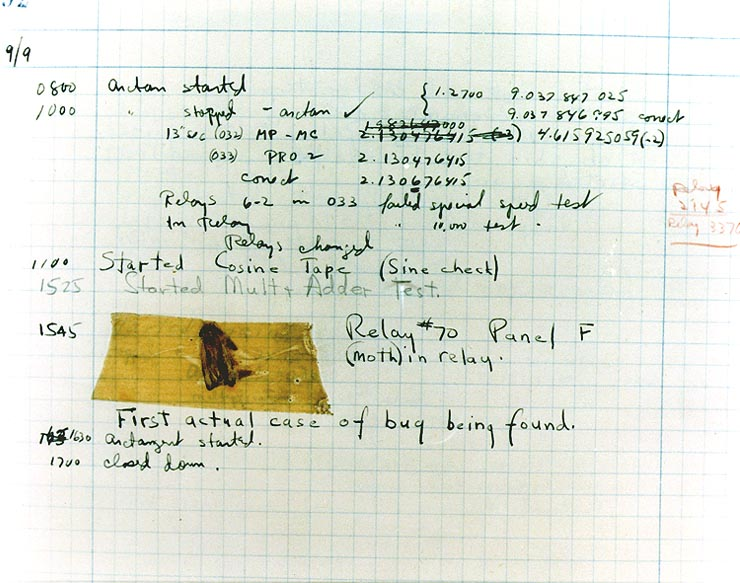
\includegraphics[width=0.8\linewidth]{debugging}
\caption{\ttfamily{'First actual case of bug being found'. September 9, 1947}}
\label{fig:Debugging}
\end{figure}

Well\ldots 

You can call me a naïve idiot, but what if into the 'Mark II' has been climbed and deadly shocked not a moth, but a cat?

\begin{quote}
Or a programmer?
\end{quote}

In fact, the term "bug" to describe defects already has been a part of engineering jargon for many decades and predates computers and computer software. It may have originally been used in hardware engineering to describe mechanical malfunctions. 

For instance, \rindex{\textbf{T}!Thomas Edison}Thomas Edison wrote the following words in a letter to an associate in 1878\footnote{~Edison to Puskas, 13 November 1878, Edison papers, Edison National Laboratory, U.S. National Park Service, West Orange, N.J., cited in Hughes, Thomas Parke (1989). American Genesis: A Century of Invention and Technological Enthusiasm, 1870-1970. Penguin Books. p. 75. ISBN 978-0-14-009741-2.}:

\begin{quote}
    It has been just so in all of my inventions. The first step is an intuition, and comes with a burst, then difficulties arise~\textemdash~this thing gives out and [it is] then that "Bugs"~\textemdash~as such little faults and difficulties are called~\textemdash~show themselves and months of intense watching, study and labor are requisite before commercial success or failure is certainly reached.
\end{quote} 

In '40 every computer guy was a radio mechanic or somehow similar to it (you cannot operate an old fashioned computer without being able to repair it several times by a day by your own hands and an soldering iron). So, computer operators were already familiar with the engineering term 'bug'. They amusedly kept the insect in the computer log, because it is really fun to discover a personalization of 'a bug'. That's why they noted it as the "\textit{First actual case of bug being found}" :)

\begin{quote}
Today this log book, complete with attached moth, is part of the collection of the Smithsonian National Museum of American History.

Why a log: on those days every interaction with the computer had to be noted on a paper.                                                                                        \end{quote} 

And Grace Hopper did not find the bug, as she readily acknowledged that. The notation "\textit{First actual case of bug being found}" was made by a group of computer operators, including William "Bill" Burke~\textemdash~maybe he wrote the famous sentence.

And the date in the log book was September 9, 1947, not 1945. The related term "debug" also appears to predate its usage in computing: the Oxford English Dictionary's etymology of the word contains an attestation from 1945, in the context of aircraft engines.

\section{Bug Reporting}
\label{sec:Bug Reporting}

The process of explaining the steps, which lead to the bug happens. This notice with a proven screenshot should be stored in a bug-tracking system [p.\pageref{sec:Bug Tracking System}].
\section{Bug Tracking System}
\label{sec:Bug Tracking System}

Any software that facilitates the collaborative recording and status tracking of defects and changes.

Usually the \url{https://www.atlassian.com/software/jira} system is used for this.

\begin{quote}
In fact, \index{Jira}Jira is not a bug-tracking system, it's a Task-tracking system. but any defect recorded can be viewed as a 'task for fixing', so nobody cares.                                                                                                                                                       \end{quote} 

I'll preffer \url{https://www.mantisbt.org/}.

Choose your own Bug Tracker.
\section{Bug Verification}
\label{sec:Bug Verification}

\rindex{\textbf{B}!Bug Verification}A process, where the tester try to reproduce on new build each bug, which was reported by developers as 'Fixed'.

\section{Build}
\label{sec:Build}

\rindex{\textbf{B}!Build} \rindex{\textbf{V}!Version}A compiled version [p.\pageref{sec:Version}] of a program. 

\begin{quote}
Any program.
\end{quote} 

It comes from the \url{https://en.wikipedia.org/wiki/Software_versioning}.

\section{Change Management}
\label{sec:Change Management}

\index{Change Management}This is an approach to controlled way to effect a change, or a proposed change, to a product or service.

It is not only about software testing. But if you tend to be a manager in testing area\ldots\footnote{~See a nice 'How-to introductory guide' to Change management area at \url{http://www.change-management.com/how-to-guide.htm}}

\subsection{'Change management' principles}
\label{sec:'Change management' principles}

        \begin{enumerate}
\item 
At all times involve and agree support from people within system (system = environment, processes, culture, relationships, behaviors, etc., whether personal or organizational).
\item 
        Understand where you/the organization is at the moment.
\item 
        Understand where you want to be, when, why, and what the measures will be for having got there.
\item 
        Plan development towards above No.3 in appropriate achievable measurable stages.
\item 
        Communicate, involve, enable and facilitate involvement from people, as early and openly and as fully as is possible.                                                                                                                             \end{enumerate}

\section{Change Request}
\label{sec:Change Request}

\index{Change Request}A formal proposal for an alteration to some requirements or functions.

Often arises when the client want an addition (or alteration) to the agreed-upon deliverables for a project. Such a change may involve an additional feature or customization or an extension of service, among other things. So it had to be analyzed apart.

Because change requests are beyond the scope of the agreement, they generally mean that the client will have to pay for the extra resources required to satisfy them.
\section{Checklist-based Testing}
\label{sec:Checklist-based Testing}

\index{Checklist-based Testing}Stupid term, but it is very human\ldots

If you need to dig a hole in the mother Earth, you will need a spade. And the process of creating a hole will be called 'to dig', not something like 'spade digging'. Because it doesn't matter, how you will dig a hole. You will use a spade, of course. Or your hands.

When you will use in testing a checklist, this is still the same testing, right?!

But if you want to feel yourself less dumb, you can say, that you will use the \textbf{Checklist-based Testing}. Something unusual! Something great! A new type of testing!

And if someone will interfere, just tell him following magic words: \russianq{\textit{A checklist-based Testing is a test design technique whereby the experienced tester uses a high-level list of items to be noted, checked, or remembered, or a set of rules or criteria against which a product has to be verified. Step aside, whiffet!}}

All the chicks will starve to death admiring you, my ass.

\section{Compatibility Testing}
\label{sec:Compatibility Testing}

\index{Compatibility Testing}This is a part of non-functional testing. During this type of testing we try to understand, if the tested application is compatible with the computing environment or other specified application.

For example, an app designed to retrieve data from Internet should be compatible with all type of networks. Or an app, designed to work with Excel 97 format (.xls) should work with \index{MS Excel}Excel 2010 format (.xlsx)

Often you will hear about \index{Firefox}Browser compatibility testing, which can be more appropriately referred to as user experience testing, but anyway. This requires that the web applications are tested on different web browsers, to ensure the following:

\begin{itemize}
\item 
    Users have the same visual experience irrespective of the browsers through which they view the web application.
\item 
    In terms of functionality, the application must behave and respond the same way across different browsers and sometimes~\textemdash~operating systems.
\item 
    Hardware (different phones and applications).                                                 \end{itemize}

\section{Component Testing}
\label{sec:Component Testing}

A \rindex{\textbf{C}!Component Testing}\textbf{Component} is an abstract common term. We suppose here any minimal software item that can be tested in isolation, without interaction with any other software items.

\begin{quote}
E.g., user only can create new profile, but all other functions like setup user avatar or name are unavailable (or are not tested for some reason). The user profile is just a Component from the System point of view, and inside of this Component the ability to add an avatar is just a Component too.

Your finger is a component of your hand. And your hand is a component of your body. And your body is a component of your country. 

Any complex System can be just a component of any other System.\end{quote} 

\textbf{Component Testing} is aimed at verification of the correct work of \textbf{individual} software components, such as specific functional areas or/and features (or sub-features) without ensure that any other components works as expected.

It may include the \rindex{\textbf{F}!Function Testing}functional testing, as well as testing of designs and content of the features or/and functional areas.

The \textbf{strong side} of this approach is obvious~\textemdash~the component can be tested from A to Z.

Common \textbf{weakness} of this approach: apart some components can work as expected, but then they are engaged in a system, they can interfere with other components and some unexpected defects may appear. That's why only component testing will never be enough.

Usually internet shops are deployed as a bunch of components, which are already integrated. This means, that a clear isolation of some Components for testing purposes cannot be achieved. That's fine, because we always provide our shops packed with all amount of functionality.

\section{Continuous Integration (CI)}
\label{sec:Continuous Integration (CI)}

\rindex{\textbf{C}!Continuous Integration (CI)}In software engineering this is a practice of merging all developer working copies with a shared mainline several times a day.

It was first named and proposed as part of extreme programming (XP). Was originally intended to be used in combination with automated unit tests written through the practices of test-driven development.

Initially this was conceived of as running all unit tests and verifying they all passed before committing to the mainline. This helps avoid one developer's work in progress breaking another developer's copy. If necessary, partially complete features can be disabled before committing using feature toggles.

Continuous integration isn't universally accepted as an improvement over frequent integration. 

\section{Cost of Quality}
\label{sec:Cost of Quality}

\index{Cost of Quality}This is a calculation of the total cost of quality-related efforts and deficiencies. The results of such calculations sometimes lead to sever managerial decisions at the whole Project scale.

It was first described by \index{Armand Feigenbaum}Armand Feigenbaum in a 1956 Harvard Business Review article.

Cost of Quality is the total costs incurred on quality activities and issues and often split into prevention costs, appraisal costs, internal failure costs and external failure costs.

If you don't know how much \$\$ costs the last founded Defect, then you cannot know the Cost of Quality on your Project.

Advanced in the Project, this amount grows, because with the time each Project engage more and more software, time and materials. Sometimes managers try to reduce the cost of quality without reduce the quality. Well, sometimes this help a lot. Sometimes this is not the smartest decision. It depends of...

Check the 'Cost of poor quality' ideas \url{https://en.wikipedia.org/wiki/Cost_of_poor_quality}.
\section{Coverage}
\label{sec:Coverage}

\index{Coverage}The degree, expressed as a percentage, to which a specified coverage item has been exercised by a test suite.
\section{Criteria}
\label{sec:Criteria}

\rindex{\textbf{C}!Criteria}A standard of judgment or criticism. 

Or a rule or principle for evaluating or testing something.

\section{Debugging}
\label{sec:Debugging}

\index{Debugging}A process, where developers start to prove their best skills.

The debugging is not the process of fixing bugs. Usually it looks like someone deliberately send to a program data with errors, trying to figure out where the calculation will be incorrect. When a weak point will be discovered, then the bug-fixing will begin.

In ancient times (1940-1970) the debugging was the primary testing approach. Those programmers had to understand clearly what (and how) the computers doing their job. And they act respectively.
\section{Decision Table Testing}
\label{sec:Decision Table Testing}

\index{Decision Table Testing}An excellent logical tool to capture certain kinds of system requirements and to document internal system design. 

They are used to record complex business rules that a system must implement. 

They can serve as a guide to creating test cases. Decision tables are a vital tool in the tester's personal toolbox.

Not every analyst, designer, programmer and/or tester are familiar with this technique\footnote{Quote from <<A Practitioner's Guide to Software Test Design>> by \index{Lee Copeland}Lee Copeland, 2004, Artech House, Inc.}.

Sad but true.
\section{Defect}
\label{sec:Defect}

\index{Defect}A flaw in a component or system that can cause the component or system to fail to perform its required function, e.g. an incorrect statement or data definition.

Usually we name it \index{Bug}Bug [p.\pageref{sec:Bug}].

\subsection{Defect Management}
\label{sec:Defect Management}

This is a process of

\begin{itemize}
\item 
    recognizing,
\item 
investigating,
\item 
taking action
\item 
and disposing of defects.                             \end{itemize}

It involves recording defects, classifying them and identifying the impact on the project or tested application.

\subsection{Defect Report}
\label{sec:Defect Report}

A document (an item in \index{Jira}Jira) reporting on any flaw in a component or system that can cause the component or system to fail to perform its required function.

\subsection{Priority and Severity}
\label{sec:Priority and Severity}

Consider the impact of Defect at the whole system. 

And here is two terms for this classification: 

\subsubsection{Severity}
\label{sec:Severity}

\begin{description}
\item[Critical]~\textemdash~such severity is assigned when you lose the ability to work with the System because a Bug happens. You have lose information, or the Product cannot do his main task, or the Device is reset because of overloading... Almost every Bug at Checkout is Critical :)

\item[Major] – well, you can somehow continue to work, or you can switch to another task, but the system is seriously affected by this Bug.

\item[Minor] – bug is available, but it does not adversely affect the Product functionality.                                                                                     \end{description}

Who is charged with authority to set the Severity? 

First of all~\textemdash~the tester, who had discovered the Bug. 

Second~\textemdash~the team lead. 

Or the Manager. 

Or the Client itself.

\subsubsection{Priority}
\label{sec:Priority}

The level of business importance assigned to an item, e.g. defect.

For example, on our site user can buy some cool stuff, and on the checkout the field 'Provide your credit card info' is missed. This is a Critical bug with High priority.

Or on our site user can buy some cool stuff, and on the checkout the field 'Provide your credit card info' is available, but is named 'Provide your credit card info hzhzhzhzhzh'. This is a Major bug with High priority.

Or on our site user can buy some cool stuff, and on the checkout the field 'Provide your credit card info' is available, but is named 'Provide your credit card' instead of 'Provide your credit card info'. This is a Minor bug with High priority.

Or on our site user can buy some cool stuff, and they can download our worldwide stores list, but the file is missed on the file server. This is a Major bug with Minor priority. Yes, this is a bug, it is important, but we will fix it when we will have enough time. Forget about it\ldots

\section{Defect-based Test Design Technique}
\label{sec:Defect-based Test Design Technique}

\index{Defect-based}Well, this is not a technique (an approach, I suppose), but it's worthing your attentive attention.

If you will focus on searching defects, not on checking if requirements are implemented — what will you see?

When the target defects are determined based on taxonomies (a \index{Taxonomy}Taxonomy is a hierarchical list) that list root causes, defects, and failures, adequate coverage is achieved when sufficient tests are created to detect the target defects and no additional practical tests are suggested.

\textbf{Example}: list some potential defects for your app. Or make some assumptions, like 'User add several items to cart, and each entry will not disappear with each new item added' and — check it out. If this will happen for real — hooray, you just supposed a bug and you really made him discovered! 

If not — suppose something else, and check it out.

This approach is far, far away from reading basic requirements, add an item to cart, as expected, and declare, that everything is ok.
\section{Development Environment}
\label{sec:Development Environment}

\index{Development Environment}A dev environment is any infrastructure, where the developers has the full authority to make any changes they needed.

Opposite is the \index{Testing Environment}Testing Environment. This can be a server with a full replication from Development server, but only QA makes decisions about the updating anything on their environment.

By the way, the software, aims to help in programming is a Development Environment too. But it is called 'Integrated Development Environment'.

\begin{quote}
E.g., the \index{Eclipse}'Eclipse' is an IDE (Integrated Development Environment). And \index{IntelliJ IDEA}'IntelliJ IDEA'  is an IDE (Integrated Development Environment). And even \index{MS Excel}MS Excel can be an IDE for VisualBasic developers. 
\end{quote} 
\section{Development of Test Cases}
\label{sec:Development of Test Cases}

This is the best process in the testing work! 

Development, development, development, development, development, development, development, development, development of \index{Test Case}Test Cases!

Can be done in a very clever way\footnote{The righteous way.}.

Or in a very dumb way.
\section{Documentation Testing}
\label{sec:Documentation Testing}

\rindex{\textbf{D}!Documentation Testing}A confusing term. There are no reason for test the documentation. Use it in testing, that's all!

Just grab \rindex{\textbf{R}!Requirements}requirements and think:
\begin{itemize}
 \item what should be implemented,
 \item what can be tested.
\end{itemize}

\begin{figure}[!h]
\centering

\includegraphics[width=0.8\linewidth]{no-app-for-that}
\caption{\ttfamily{'Sorry, son\ldots there's no app for that'}}
\label{fig:no-app-for-that}
\end{figure}

You will need only \rindex{\textbf{N}!Notepad} Notepad and your own imagination for this.

Note all your ideas and questions, search for answers, and repeat steps one by one (this is an incremental task) till the end of your career in testing.

\section{Domain Analysis Testing}
\label{sec:Domain Analysis Testing}

\index{Domain Analysis}A very mature test design technique.

Used to identify efficient and effective test cases when multiple variables can or should be tested together.

Implies a lot of equivalence partitioning and boundary values analysis, so a junior tester will never be able to do it.

Not every Senior Tester is familiar with this advanced approach to design test cases either.

Sad but true.
\section{End-to-end Testing}
\label{sec:End-to-end Testing}

\rindex{\textbf{E}!End-to-end Testing}A convenient expression for establish the complexity of system being to test and the nature of test cases, designed for this.

Consider a platform, where individual component systems are integrated with each other, so a new shop (a new system) can be created without having to develop applications from new. Complexity of such software requires to test whether the flow of an application is performing as designed from start to finish.

Example~\textemdash~Promotions. Every step can be tested apart, but it is more important to be sure that the whole process (create and apply new Promotion) works as expected.

The purpose of carrying out end-to-end tests is to identify system dependencies and to ensure that the right information is passed between various system components and systems.

Someone can act such type of testing like very annoying. Well, complex thing requires complex testing.

\section{Entry and Exit Criteria for Testing}
\label{sec:Entry and Exit Criteria for Testing}

\begin{quote}
Understand what is a \index{Criteria}Criteria first [p.\pageref{sec:Criteria}].
\end{quote} 

Sometimes is very hard to agree about when we can start or stop testing.

For example, developers already had developed something, and \index{Customer}Client call us to start testing. In his opinion, this is enough for starting testing — here are some functionality, just use your imagination and common sense and go on. But we still have no requirements, and we cannot be sure, that we are on the same page with developers about what and how should work. Can we just shut up and let's the mortal testing begin, or we will hang on our hands and refuse to start, because we had no time for preparation, no test cases, no requirements\ldots?

Yes, if we have common sense and we can discuss with our customer any issue, we can start without any requirements and fears.

But if the Customer is \index{Mafia}Al Capone itself, and in case of something will fail on our website you will wake up in the morning being silently buried in a black box under the heavy ground\ldots We need to agree something before the process will start.

Entry/exit Criteria for Testing are a set of generic and specific Conditions discussed between the client and executor. This criteria doesn't exist as a law, and always can be/should be revisited.

\subsection{Entry criteria for testing}
\label{sec:Entry criteria for testing}

\index{Entry criteria}The purpose of Entry criteria is to prevent a task from starting which would entail more (wasted) effort compared to the effort needed to remove the failed entry criteria.

Entry criteria for testing can be following:

    \begin{itemize}
\item 
for each functionality we have a requirement available,
\item 
    we have enough human resources for the testing process,
\item 
    all third-party units are available for being used with our system under test,
\item 
    build is frozen and no new functionality will be added or changed...                                                                        \end{itemize}


\subsection{Exit criteria for testing}
\label{sec:Exit criteria for testing}

\index{Exit criteria} The purpose of Exit criteria is to prevent a task from being considered completed when there are still outstanding parts of the task which have not been finished. Exit criteria are used to report against and to plan when to stop testing. 

Exit criteria for testing can be following:

    \begin{itemize}
\item     all critical functionality was tested and here is the complete report,
\item     all discovered critical bugs was fixed and retested,
\item     the time for testing is out...\end{itemize}

By the way, sometimes \textbf{Exit Criteria} for Testing is called as \textbf{Completion Criteria}.
\section{Equivalence Class Testing}
\label{sec:Equivalence Class Testing}

\begin{quote}
\index{Equivalence Class Testing}This should be called \textbf{Equivalence partitioning of test cases}, but nobody cares.\end{quote} 

Don't pretend that this technique can be used to reduce the number of test cases without lowering the test coverage, because reducing test cases always lower the test coverage level. Automobiles was created for consuming petrol or for carrying human beings from the maternity hospital to the cemetery as fast as possible?

\subsection{Class}

A \index{Class}class is a group of some items with some common attributes, characteristics, qualities, or traits. 

Grouping is useful for science, it helps to discuss as single entities whole classes, not separate items.

Trick is that \emph{one item} can inherit different characteristics and qualities  \emph{at the same time}. For example, an usual \emph{man} can be added to several groups (classes) simultaneously: 

\begin{itemize}
 \item 
 human being
 \item 
 bus driver
 \item 
 pig
 \item 
 father
\end{itemize}

\subsection{Equivalence}

There are a lot of terms for showing that two items are equal: equal, comparable, identical, correspondent, duplicate, matched, uniform.

Any two things can be called equal, if they have the exactly same attributes. 

\begin{quote}
 
\textbf{Example}: you have two brand new bottles of \index{Whiskey}whiskey. 

They exists apart in this Universe, but now they are identical, equal, the same, they duplicate each other.

If you will open one bottle, they immediately will become unequal (one is opened, the other is sealed).

But once both bottles are opened, they again become equal.
\end{quote}

Ok, this bottles cannot be called 'equal' for real. But they can be declared as 'equal' only for our convenience.

There is an \emph{meta} word for such statement: this two bottles are not equal (identical), but for the final result you can act with them like they ARE identical. This is called \emph{Equivalence}.

\begin{quote}
 
\textbf{Other example}: you should use a passenger train for travel in \index{Metro train}metro. Will matter what kind of train you will have to use? His color, capacity, length, personal number and the manufacturing year, or something like that?

No! All those DIFFERENT trains from your route WILL BE equivalent one to others, while your journey.

If you will use one of thousand trains, you can assume, that all other trains can complete the same task.

Again, all those trains are not equal one to others. Each of them has his own number, different colors, different history and brake conditions, they was released in different ages. They are not equal, they are only equivalent.
\end{quote}

Warning! Equivalence is not a substitution or something totally equal. 'Equivalence' is not 'Equality'.


\subsection{Equivalence partitioning of test cases}

An equivalence class \emph{can} consists from a set of data that is treated the same by the module or that should produce the same result. Any data value within a class is equivalent, in terms of testing, to any other value. Specifically, we would expect that if one \index{Test Case}test case in an equivalence class detects a defect, all other test cases in the same equivalence class are likely to detect the same defect.

A group of tests forms an equivalence class if you \emph{believe} that:

\begin{itemize}
\item 
They all test the same thing.
\item 
If one test catches a bug, the others probably will too.
\item 
If one test doesn't catch a bug, the others probably won't either.\end{itemize}

This approach assumes, of course, that a specification exists that defines the various equivalence classes to be tested. 

And you should clearly understand, that your 'grouping' of test cases can be formally good, but totally wrong.

The \textbf{main gap}: for example, you get your car from the car service, and the mechanic says: <<\textit{We had to check all the wheels. Well, we checked only two wheels with brakes. You know, they're all four are equivalent to each other, so we have checked out those two, they are ok, so we \emph{assume} that the remaining wheels are ok too. Have a nice day}>>. Will you have a nice day?

Divide into equivalence classes only \index{Test Case}Test cases, not the \index{Functionality}Functionality of a product.
\section{Exhaustive Testing}
\label{sec:Exhaustive Testing}

\rindex{\textbf{E}!Exhaustive Testing}A test approach in which the \rindex{\textbf{T}!Test Suite}test suite comprises all combinations of input values and preconditions.

\begin{quote}
All combinations!
\end{quote} 

As you know, nobody can test all input combinations into a modern software, so every moron knows that exhaustive testing is totally impossible.

In fact, exhaustive testing it is totally possible, but not all the time necessary. You cannot test everything. But you can predict everything that can happen with the tested software. Predictability lead to control.

\section{Exploratory Testing}
\label{sec:Exploratory Testing}

\rindex{\textbf{E}!Exploratory Testing}A very cool, but informal test design technique.

It is hard to explain this approach in a few words, because it is completely unusual for almost all testers. But it can be demonstrated and explained step-by-step (it's like riding a bicycle).

Here is the simplest explanation of this approach:

\begin{figure}[!h]
\centering
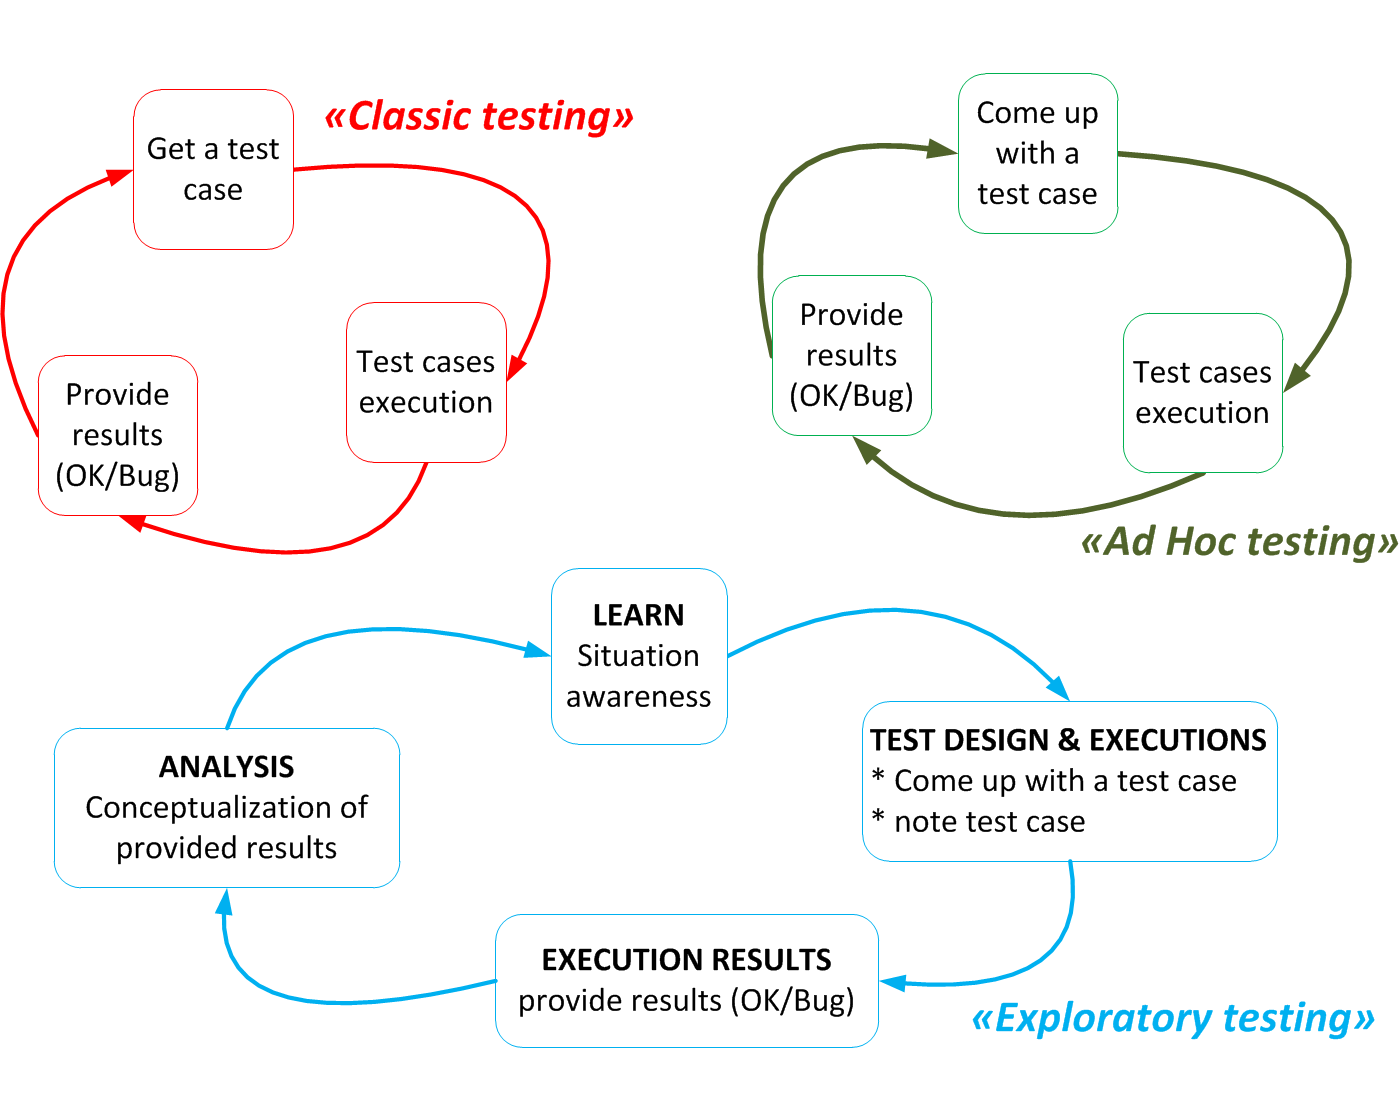
\includegraphics[width=\linewidth]{ClassicAdHocExploratoryTesting}
\caption{\ttfamily{Simple explanation of Classic \& Ad Hoc \& Exploratory testing}}
\label{fig:ClassicAdHocExploratoryTesting}
\end{figure}

\section{Feature}
\label{sec:Feature}

\rindex{\textbf{F}!Feature}An attribute of a component or system specified or implied by requirements documentation (for example reliability, usability or design constraints).

\section{Function}
\label{sec:Function}

\begin{quote}
 Cat's functions are 'to make purrrr' and to hunt mouses.
\end{quote} 

The \textbf{Function} is what a given entity does in being what it is.

So, the \textbf{Functionality} is an ability of software to perform a task.

Word is taken from the Latin "\textit{functio}" - to perform.
\section{Functional Requirement}
\label{sec:Functional Requirement}

\rindex{\textbf{F}!Functional Requirement}In programming a Function is a named section of a program that performs a specific task.

In the same way that a File is a named section of some data on your hard-disk drive.

\begin{quote}
The term function is also used synonymously with operation and command. For example, you execute the 'delete' function to erase a word.
\end{quote} 

A \textbf{Function}, in its most general use, is what a given entity does in being what it is [p.\pageref{sec:Function}].

The \textbf{Functionality} is an ability of software to perform a task.

A \textbf{Functional Requirement} is an abstract, which describes the functionality task that a software system should \textbf{do} for the user needs.

\begin{quote}
And a Non-functional requirements usually place constraints on \textbf{how} the system will do so. See [p.\pageref{sec:Non-functional Requirement}] for details.                                                                                        \end{quote} 

An \textbf{example} of a functional requirement would be that a system must send a an email whenever a certain condition is met (e.g. an order is placed, a customer signs up, etc).

\begin{quote}
A related non-functional requirement for the system can be that emails should be sent with a latency of no greater than 12 hours from such an activity.
\end{quote} 

Then \textbf{Functional Requirements} are done, it's time to write \textbf{Functional Specifications}.

You understand the difference between Requirements and Specifications?

\section{Functional Specification}
\label{sec:Functional Specification}

\index{Functional Specification}This is an extention of a Functional \index{Requirements}Requirement [p.\pageref{sec:Functional Requirement}].

\textbf{Functional Requirement} is an abstract, which describes \emph{what} a software system should do from the user point of view.

\begin{quote}
 I want to have a red car for driving on the streets.
\end{quote} 

\textbf{Functional Specification} describes \emph{how exactly} the functional requirement will be implemented.

\begin{quote}
 I want to have a car painted in \#ff0000 with engine 1.6 and McPherson suspension.
\end{quote} 
\section{Functional Testing}
\label{sec:Functional Testing}

\rindex{\textbf{F}!Functional Testing}Any testing based on an analysis of the specification of the functionality of a component or system.

The functional testing will be executed to evaluate the compliance of a system or component or third-party with specified functional \rindex{\textbf{R}!Requirements}requirements and corresponding predicted results.

Functional testing is performed for each planned feature and is guided by approved by \rindex{\textbf{C}!Customer}client requirements.

\section{Impact Analysis}
\label{sec:Impact Analysis}

\rindex{\textbf{I}!Impact Analysis}In fact, this should be named \textbf{Change impact analysis}, but anyway~\textemdash~this is a method to identify the potential consequences of a change in a complex system.

Consider \rindex{\textbf{N}!Notepad}'Notepad' as a simple software under test. We can add new functions (or modify existed). We would like to set assure, that this change will not alter existed functions. How?

We can proceed to regression testing (consider the level of boring testers and costs). Or we can setup a table, where we will trace all Notepad functionality and their junction points.

Now, we can see, which functionality will be affected by changes, and can retest only areas, where changes will have the impact.

Problem with this impact tables is the same as for any other project documentation~\textemdash~they should be updated on a regular basis.

And yes, if the project is short or 'small'~\textemdash~we can omit such documents.

\section{In Scope / Out of Scope}
\label{sec:In Scope / Out of Scope}

A 'scope' is an abstract term for setting the area or subject relevant for the discussion.

\begin{quote}
For example, two men meet for a coffee. For sure, they will start to discuss business issues, and only business issues will be in scope of their conversation. Any other stuff (cars, pets, women) will be 'out of scope'.

But when this two will have to exterminate the second bottle of \rindex{\textbf{W}!Whiskey}'Johnnie Walker', business issues will become 'out of scope', and chat will be oriented to cars, women, pets and other important for business issues.                                                                                                                                                                                                                     \end{quote} 

Same thing relate to testing: testers have to establish from the start which functionality will be tested during next testing session; they should list all functions 'in scope' and all the functions, which will not be tested during this session, and agree with Development and Client about why this will be and those will not be tested.

\begin{quote}
By the way, such documents are called Testing Scope and they are an indispensable part of any \rindex{\textbf{T}!Test Plan}Test Plan.\end{quote} 

Why testers must define the Testing Scope? This should be done especially to cover testers heads in case of strange questions appears, like '\textit{But why this and those things wasn't tested?}'. 

Sometimes testers can save their lives with this 'in scope' and 'out of scope' lists.

Sometimes not.

\section{Integration Testing}
\label{sec:Integration Testing}

\rindex{\textbf{I}!Integration Testing}Integration testing is a process, where different parts of system under testing are engaged one by another.

Such testing is done to ensure that all engaged components (may be included third-parties) maintain data integrity and can operate in coordination with other system artifacts in the same environment.

This type of testing is performed to expose defects in the interfaces and in the interactions between integrated components or systems. There are a huge possibility, that each software component can be bugless apart, but on the integration phase can appear some bugs, that cannot be imagined, supposed and identified. They can be discovered only at the Integration testing phase.

\section{Item Pass/Fail Criteria}
\label{sec:Item Pass/Fail Criteria}

\begin{quote}
Understand what is a \rindex{\textbf{C}!Criteria}Criteria first [p.\pageref{sec:Criteria}].
\end{quote} 

\textbf{Pass/Fail Criteria} will be used to ensure the completeness of the test process.

It sound very obvious, but try to explain your judgement about '\textit{How do you know, that the testing of Change Avatar in User Profile is done?}' Sometimes is very easy to understand this (I can change user Avatar, all satisfied citizens are going home). But sometimes not.

\begin{quote}
Where is the previous user Avatar picture? It is still available, but was marked as 'Deleted'? Or it was completely deleted from file server?
\end{quote} 

\section{Iterative Development Model}
\label{sec:Iterative Development Model}

Check \href{http://en.wikipedia.org/wiki/Iterative_and_incremental_development}{Iterative and incremental development}\footnote{~\url{http://en.wikipedia.org/wiki/Iterative_and_incremental_development}} article in wikipedia, please. There are nice pictures too.

Iterative Development ModelIterative and Incremental development is any combination of both iterative design or iterative method and incremental build model for software development. This process may be described as an 'evolutionary acquisition' or 'incremental build' approach.

The relationship between iterations and increments is determined by the overall software development methodology and software development process. The exact number and nature of the particular incremental builds and what is iterated will be specific to each individual development effort.

Iterative and incremental development are essential parts of the Modified waterfall models, Rational Unified Process, Extreme Programming and generally the various agile software development frameworks.

It follows a similar process to the 'plan-do-check-act' cycle of business process improvement.

\section{Maintenance of Test Cases}
\label{sec:Maintenance of Test Cases}

\rindex{\textbf{M}!Maintenance of Test Cases}Maybe, the most annoying process for every smart tester in the world.

\rindex{\textbf{R}!Requirements}Requirements (and Expectations) in a Product can happen many times during a product development lifecycle, so \rindex{\textbf{T}!Test Case}test cases can become totally obsolete. Rewrite them all, or write new test cases.

What would you do with this issue?

Real challenge, huh?

\section{Metaphor}
\label{sec:Metaphor}

A \rindex{\textbf{M}!Metaphor}\emph{Metaphor} is a figure of speech that refers, for rhetorical effect, the attributes of one thing by mentioning another thing.

It may provide clarity or identify hidden similarities between two ideas. A \textit{Metaphor} directly equates this two items, and does not use "like" or "as" as does a \textit{Simile}. 

Example: 

\begin{verse}
The moon has looming over the horizon like\footnote{~Yeah, the word "like" was used, but anyway} a big orange. 
\end{verse} 

From the other side, nobody will understand the same metaphor, used vice versa:

\begin{verse}
An orange has lying on a plate, like a moon over the horizon. 
\end{verse} 

Sound stupid, isn't it?

Some methapors works perfect in both sides, some not.

\section{Migration Testing}
\label{sec:Migration Testing}

\rindex{\textbf{M}!Migration Testing}Consider that a company switch from one DBMS to another (from MySQL to Oracle). Or the architecture of DB requires a massive innovation. Then will be required a database Migration testing.

Database migration may be done manually, but it is more common to use an automated ETL (Extract-Transform-Load) process to move the data.

Database migration testing may encounter problems when:
\begin{enumerate}
 \item The data in the source database(s) changes during the test;
 \item Some of the source data is corrupt;
 \item The mappings between the tables/ fields of the source databases(s) and target database are changed by the database development/ migration team;
 \item A part of the data from the source database is rejected by the target database;
 \item Data migration takes too long because the database migration process is too slow or the source data file is too large.
 \end{enumerate}
 
 The test approach for database migration testing consists of the following activities:
 
\begin{enumerate}
 \item  
 Design the validation tests. In order to test database migration, SQL queries are created either by hand or using a tool, such as a query creator. The test queries should contain logging statements for the purpose of effective analysis and bug reporting after the tests are complete.
 \item Set up the test environment. The test environment should contain a copy of the source database, the ETL tool (if applicable) and a clean copy of the target database. The test environment should be isolated so that it is not changed externally during the tests.
 \item Run your validation tests Depending on the test design, the database migration process does not need to completely finish before starting tests.
 \item Report the bugs.
 \end{enumerate}

\section{Monkey Testing}
\label{sec:Monkey Testing}

\rindex{\textbf{M}!Monkey Testing}A metaphor for naming the producer of any input for a program.

The name 'monkey' comes from the the 'Infinite monkey'\footnote{~\url{http://en.wikipedia.org/wiki/Infinite_monkey_theorem}} theorem. There is an adage that ‘\textit{thousand monkeys at a thousand typewriters will eventually type out the entire works of \rindex{\textbf{W}!William Shakespeare}Shakespeare}’.

\begin{figure}[!h]
\centering

\includegraphics[width=0.8\linewidth]{shakespeare}
\caption{\ttfamily{This is Shakespeare. He looks at you as at an infinite monkey}}
\label{fig:shakespeare}
\end{figure}

For example, a monkey test can enter random strings into text boxes to ensure handling of all possible user input or provide garbage files to check for loading routines that have blind faith in their data. The test monkey is technically known to conduct \rindex{\textbf{R}!Random Testing}Random testing.

\section{Negative Testing}
\label{sec:Negative Testing}

\rindex{\textbf{N}!Negative Testing}A test designed to determine the response of the system outside of normal parameters.

It is designed to determine if the system performs error handling with an other than expected input.

Understand, that when you check something like 'Enter following abracadabra and system should explain that there is an unaccepted symbol, please enter data without errors'~\textemdash~this is \rindex{\textbf{P}!Positive Testing}Positive Testing [p.\pageref{sec:Positive Testing}], because you have the expectations about systems response.

\section{Non-functional Requirement}
\label{sec:Non-functional Requirement}

A \index{Requirements}requirement that does not relate to functionality, but to attributes such as reliability, efficiency, usability, maintainability and portability.

Typically non-functional requirements fall into areas such as:
\begin{itemize}
\item 
Accessibility
\item     Capacity, current and forecast
   \item  Compliance
    \item Documentation
  \item   Disaster recovery
    \item Efficiency
    \item Effectiveness
    \item Extensibility
   \item  Fault tolerance
    \item Interoperability
   \item  Maintainability
   \item  Privacy
   \item  Portability
   \item  Quality
  \item   Reliability
   \item  Resilience
   \item  Response time
    \item Robustness
   \item  Scalability
  \item   Security
   \item  Stability
  \item   Supportability
   \item  Testability               \end{itemize}

\begin{quote}
How you will test the Effectiveness of \index{MS Word}MS Word processor? :)
\end{quote} 

Non-functional requirements are sometimes defined in terms of metrics (something that can be measured about the system) to make them more tangible. For example, the Effectiveness of MS Word processor can be described binary — it is effective or not. Or it can be described, for example, from 1 to 10 points.

Suppose the level of user excitement when he drive an Cadillac Eldorado 1959 — this is a non-functional requirement.

Suppose the level of user annoying when he use an app, which crashes each time when wi-fi connection is down for a second — this is a non-functional requirement.

\subsection{Non-functional Testing}
\label{sec:Non-functional Testing}

Testing the attributes of a component or system that do not relate to functionality, e.g. reliability, efficiency, usability, maintainability and portability.
\section{Pair Testing}
\label{sec:Pair Testing}

Sometimes more than one human beings work together on a single task. If the task is about testing something~\textemdash~welcome to \index{Pair Testing}Pair testing.

One does the testing and the other analyzes or reviews the testing. They can always switch their roles.

Pair Testing can significantly speed up the testing. One person is a \textbf{Driver}, second is a \textbf{Navigator}. 

\begin{figure}[!h]
\centering

\includegraphics[width=0.8\linewidth]{navigator}
\caption{\ttfamily{Beyond the limits}}
\label{fig:Navigator}
\end{figure}

Both minds can generate testing ideas, and immediately execute them. While Navigator stay for make a note about what was doing and the results, Driver can run and generate next idea, and so on. This can be done between one tester and developer or business analyst or between two testers with both participants taking turns at driving the keyboard. No limits, really!

This approach come from \index{Exploratory Testing}Exploratory Testing area [p.\pageref{sec:Exploratory Testing}], and it's very controversial. From the manager's point of view, Pair Testing looks like TWO working units do ONE job, so one testing task costs double. While this, will be better if those TWO working units were doing at the same time TWO testing tasks. 

For sure, this if very OK, when the task is to dig a hole at the land. And sometimes testing really looks like digging.

\begin{quote}
You remember the '\textit{You see, in this world there are two kinds of people, my friend: those with a loaded gun and those who dig. You dig}' © from 'The Good The Bad and the Ugly' movie? 

We must understand and admit this truest statement.                                                                                                                                                                                                                                                 \end{quote} 

But there are a lot of tasks in testing, when we need more brains for work, than hands. For such tasks \index{Pair Testing}Pair Testing can be a wonderful approach, where TWO smart people can work as ONE unit best and quicker than two working units apart.

At the end of Pair Testing this two persons survive so many challenges, that as a nice persons, they have to marry each other, so be careful with this software development technique.

\section{Pairwise}
\label{sec:Pairwise}

\index{Pairwise}A powerful test design technique. Test cases are designed to execute all possible discrete combinations of each pair of input parameters. 

It can significantly reduce the number of all combinations of variables to test all pair combinations.

Usually this powerful technique is used as a waste of time with respective attitude. Please, do not try it at home. You can fake that you totally understand what is talking about.
\section{Performance Testing}
\label{sec:Performance Testing}

Initially, \index{Performance testing}\emph{Performance} is an activity that a person does to entertain an audience, such as singing a song or acting in a play on a Broadway.

In technical language, \emph{Performance} is the ability of a mechanism to do an required action (or activity). It can be evaluated only as a numerical value.

\begin{quote}
\textbf{Example}: the old Cadillac Eldorado 1953 engine, we have reached a level of 100 km/h in 42 seconds, and this was possible because of 210 horsepower expected and available.

Performance can be evaluated, varied and measured in follow mode: 'Let's find out, if will be possible to reach a level of 100 km/h in 32 seconds at the old Cadillac Eldorado 1953 engine, if we will setup 240 horsepower instead of 230'.

Performance can be evaluated, varied and measured in follow mode 'Let's find out, how much time the old Cadillac Eldorado 1953 engine will work, if we will put a brick on the accelerator pedal and will have to wait'.
\end{quote} 

\subsection{Load \& Stress testing}
\label{sec:Load and Stress testing}

Performance testing simply implies \textbf{Load} and \textbf{Stress} testing. Difference between this testing types is logical and lies in the fact that different types of performance testing answer to different business questions.

\begin{quote}
\index{Load testing}Load testing help us to understand the behavior of the system under a specific \textbf{expected} load.

\index{Stress testing}Stress testing is normally used to understand the \textbf{upper limits} of capacity within the system.                                                                                             \end{quote} 

\textbf{Example}: there are an application with DB based on the MySQL. MySQL is a popular choice of database for use in web applications, an open-source relational database management system.

MySQL can easily support 200 hits per second (12 000 per minute, and 720 000 per hour, and 17 280 000 per day). How to test the performance of this web-site?

\begin{quote}
We can use JMeter for generate 100 hits per second. Is anything ok?

Let's generate 190 hits. Is anything ok?

Let's generate 210 hits. Is anything ok?

Let's generate 300 hits. Is anything ok?

Let's generate 500 hits. Is anything ok?

Let's generate 210 hits during 6 hours. Is anything ok?                                                       \end{quote} 

We have the same utils and we do the same things. But first it was simple Performance testing, then it became Load testing, then it became Stress testing, then it again became Load testing.

\subsection{Reliability Testing}
\label{sec:Reliability Testing}

\index{Reliability Testing}'Reliability' is a term for testing a software's ability to function, given environmental conditions, for a particular amount of time.

For example, turn on the coffee machine and use it 100 hours without any stop. Will be some problems in the software and functionality? Will be coffee available after this 100 hours? And if Yes, then what about 200 non-stop hours? Or 1000?

\subsection{Maintenance Testing}
\label{sec:Maintenance Testing}

\index{Maintenance Testing}Is that testing which is performed to either identify equipment problems, diagnose equipment problems or to confirm that repair measures have been effective. 

It can be performed at either the system level, the equipment level, or the component level.

Maintenance testing uses system performance requirements as the basis for identifying the appropriate components for further inspection or repair.

A good testing program will maintain a record of test results and maintenance actions taken. These data will be evaluated for trends and serve as the basis for decisions on appropriate testing frequency, need to replace or upgrade equipment and performance improvement opportunities.
\section{Positive Testing}
\label{sec:Positive Testing}

This is nothing else than the \rindex{\textbf{P}!Positive Testing}main approach to testing.

Our main intention is to prove that an application will work 'as expected' on giving valid input data.

In \rindex{\textbf{N}!Negative Testing}Negative testing ([p.\pageref{sec:Negative Testing}]) our intention is to prove that positive testing did not cover some situations.

Suppose following situation: I will type an email address without '@', system should alert me about my error. What kind of testing type is that? Is that A positive or a negative one?

\section{Precondition}
\label{sec:Precondition}

\index{Precondition}Environmental and state conditions that must be fulfilled before the component or system can be executed with a particular test or test procedure.

\subsection{Postcondition}
\label{sec:Postcondition}

\index{Postcondition}Environmental and state conditions that must be fulfilled after the execution of a test or test procedure.

Warning, this is not the \index{Expected result}Expected result [p.\pageref{sec:Actual Result}].
\section{Quality}
\label{sec:Quality}

\index{Quality}The degree to which a component, system or process meets specified requirements and/or user/customer needs and expectations.

A \textit{value} to some \textit{person} at some time.
\section{Regression Testing}
\label{sec:Regression Testing}

This process is very annoying and costs are high, but we can drive it in a smart way, trough \rindex{\textbf{I}!Impact Analysis}Impact Analysis [p.\pageref{sec:Impact Analysis}].

\rindex{\textbf{R}!Regression Testing}So, every system (social, political, military or software system) should continuously expand his functional possibilities to survive. This is a \textbf{Progress}.

But with more opportunities, the more relationships appears, and the more chances to find a defect. Or not to find it. This is a \textbf{Regress}.

\textbf{Regression testing} is performed for getting know, if regression appears.

\begin{quote}
 Testing brings information, remember this simple idea?
 \end{quote} 

This activity only looks like we should test some modification in software to ensure that defects have not been introduced or uncovered in unchanged areas of the software, as a result of the changes made. In fact, 'Regression testing' can be done periodically, without any changes in software. 

\begin{quote}
Now deal with it.\end{quote} 

One of our interest is to discover negative behavior, that's why we are doomed to perform a 'Regression testing' each time when new functionality is added to a software.

And 'Regression testing' it is sometimes performed when the environment is changed.

\begin{quote}
 Environment, not software. You can call this 'Integration testing', but what kind of Integration it is, if the software still the same?
\end{quote} 

You will be a great donkey, if you will advance in 'Regression testing' having only old \rindex{\textbf{T}!Test Case}test cases, '\textit{Cause this is just a re-test, right, ma?}'. You will need new test cases because of ANY significant change in software structure.

\section{Requirement}
\label{sec:Requirement}

\index{Requirements}A condition or capability needed by a user to solve a problem or achieve an objective that must be met or possessed by a system or system component to satisfy a contract, standard, specification, or other formally imposed document.

\index{Specifications}Specification is the next step after Requirement. Requirements tells what to do, and Specification tells how to do it~\textemdash~this can be two different docs.

\section{Root Cause Analysis}
\label{sec:Root Cause Analysis}

\index{Root Cause Analysis}A root cause is an initiating cause of a causal chain which leads to an outcome or effect of interest. In short: \textit{find why someone was killed, and you can find the killer}.

Root cause analysis is a method of problem solving that tries to identify the root causes of faults or problems. A lot of developers can expect such analyse from testers, but this is insane. Root cause analysis practice solve problems by attempting to identify and correct the root causes of events, as opposed to simply addressing their symptoms. Focusing correction on root causes has the goal of \emph{preventing problem recurrence}, and here testers fails.

There are many different tools, processes, and philosophies for performing Root Cause Analysis. However, several very-broadly defined approaches or "schools" can be identified by their basic approach or field of origin: safety-based, production-based, process-based, failure-based, and systems-based.
\section{SCRUM}
\label{sec:SCRUM}

\rindex{\textbf{S}!SCRUM}The term itself comes from Rugby game, and describes a way of starting play again, in which players from each team come together and try to get control of the ball by pushing against each other and using their feet, when the ball is thrown in between their feet. 

\begin{figure}[!h]
\centering
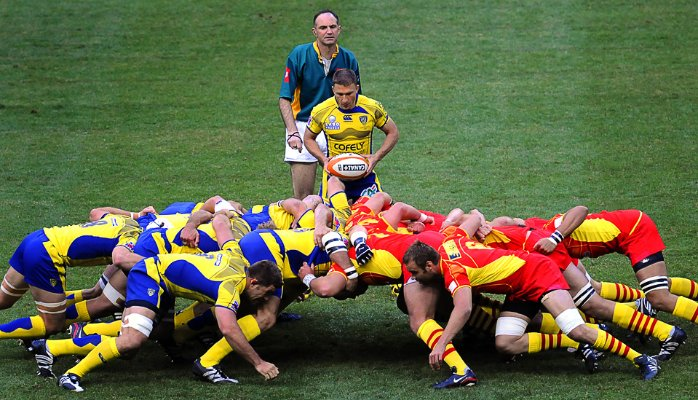
\includegraphics[width=0.8\linewidth]{realScrum}
\caption{\ttfamily{This is the real Scrum}}
\label{fig:realScrum}
\end{figure}

You can say '\textit{Jump everybody and let's kill them all!}' and millions will respond~\textemdash~yes! Well, this is \rindex{\textbf{W}!War}Rugby.

But you will suppose the SCRUM as a development approach, huh?!

\begin{figure}[!h]
\centering
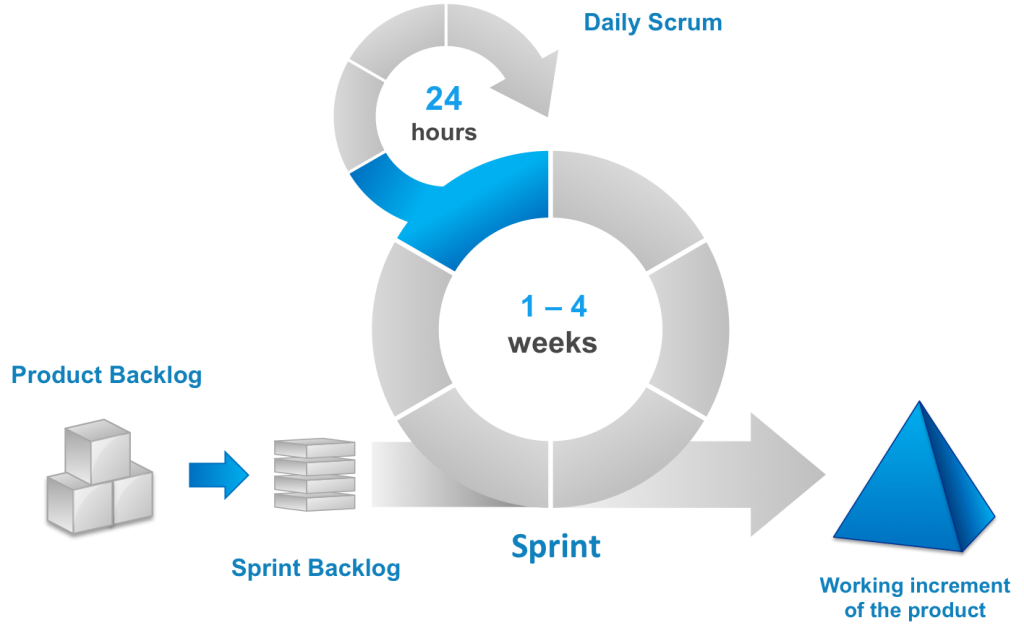
\includegraphics[width=1\linewidth]{scrumFramework}
\caption{\ttfamily{SCRUM Framework}}
\label{fig:scrumFramework}
\end{figure}

You will even say 'A software development methodology!', do you?!

This is not a methodology. 

This is a software development framework (a \rindex{\textbf{S}!Strategy}strategy) for managing product development, driven by agile principles. For being applied, the dev team already should have a development methodology.

Again, framework OVER a methodology.

\begin{verbatim}
ELSE
       Fail();
\end{verbatim}

See \rindex{\textbf{A}!Agile Software Development} Agile Software Development explanation ([p.\pageref{sec:Agile Software Development}]) \& agile principles at (\url{http://agilemanifesto.org/}) or GTFO.

\section{Security Testing}
\label{sec:Security Testing}

\rindex{\textbf{S}!Security Testing}Usually~\textemdash~a process intended to reveal flaws in the security mechanisms of an information system that protect data and maintain functionality as intended.

It looks like a simple 'Let's find some possibility to stole credit card numbers from our shop!' approach, but in fact Security Testing represent a totally different approach than testing some functionality, involving a lot of programming skills. Usually it looks like someone explore/decompile a program and write his own program for explore and decompile others.

\begin{quote}
 If you are bored for a little by \rindex{\textbf{F}!Functional Testing}Functional Testing, and you are looking for something else, then Security is the latest area for you. This is a whole profession, whis involve a lot of programming and administration servers skills and knowledge.
\end{quote} 

Well, winter is coming\ldots~Prepare for cold times. Are we enough strong for say 'Hello!' to winter? Are our bodies prepared for that?

Imagine a simple Doctor. At university he studied the human body, starting with cutting the frogs in the school laboratory, and then progressively started the autopsy of human bodies in the dissecting room.

Now suppose yourself. Do you know about medicine something more than 'If I'll get a chill, I will drink a hot tea with lemon and Aspirin!?

Feel the difference?

Who can effectively suppose/assume/find some weaknesses in human body? You, with tea and Aspirin, or a Doctor, who has killed during his university ages more frogs than you saw movies with \rindex{\textbf{B}!Bruce Lee}Bruce Lee?

Only just because it is called 'testing' (exactly like 'Functional Testing'!), each year a new generation of junior-jedi testers tries to study 'something new in testing'.

To succeed in security testing, it is necessary not only to understand how something is built, but why someone made certain technical decisions.

\section{Server}
\label{sec:Server}

A program, that can simultaneously accept a lot of references to it, put them in a queue and execute them successively, one by one.

Depending on context, the term can refer to the hardware, where the \index{Server}Server lives.
\section{Smoke Testing}
\label{sec:Smoke Testing}

\index{Smoke Testing}This is just a convenient metaphor, defining a process of superficial testing, required to being done before the real, deeper advanced testing started.

The idea consist in following: before starting to explore new build, set assure that all at least main functionality (differ from project to project) is on:

    \begin{itemize}
\item 
product catalog is available,
\item     you can add a product to cart,
\item     you can run trough checkout process,
\item     user profile are available,
\item     and so on.              \end{itemize}

If smoke testing will fail, then the whole testing process will be worthless.

If smoke testing is ok, then we can advance in testing, as expected.

Usually developers call this checking \index{Sanity Testing}'sanity testing', others (factory engineers) \index{Integrity Testing}'integrity testing'. As manual functional testers, we called it 'Smoke testing'.

\begin{quote}
A lot of years ago the testing of electronic devices started with real 'smoke testing' — plug the device to an outlet and set power 'on'.

If you see light and smoke — forget about testing, the device is broken, you will burn.                                                                        \end{quote} 

Smoke testing is always based on a subset of defined/planned \index{Test Case}test cases, that cover the main functionality of a component or system, to ascertaining that the most crucial functions of a program work, but not bothering with finer details.

A daily build and smoke test is among industry best practices.
\section{Sprint}
\label{sec:Sprint}

The term \index{Sprint}\emph{Sprint} is coming from sport. It is the act of running over a short distance at top speed.

\begin{quote}
Opposite is 'stayer'~\textemdash~a long-distance runner.\end{quote} 

Depending of physical statement, runners specialize in running on long or short distances, because this are two different strategies of running.

\begin{quote}
Sprinters runs very fast, but only at short distances (no more than 100 m). They should make an extra effort from start, immediately, without any compromises, without trying to save some power or even air breathing. Human physiology dictates that a runner's near-top speed cannot be maintained for more than 30–35 seconds due to the accumulation of lactic acid in muscles. Just get up and run!

Stayers starts slowly, at first they should try to hold on the group of all runners, at maximum saving energy. They will need all their power and speed in the latter stages of running, closer to the finish band. For example, marathon runners can run 42 km (plus ~195 m).                                                                                                                                                                                                                                                   \end{quote} 

In \index{Agile Software Development}Agile Software Development ([p.\pageref{sec:Agile Software Development}]) the term 'sprint' means almost the same~\textemdash~a short-time activity (typically one week long), where all the people involved in a project, being focused on development of some task for the project, give maximum of their power and attention.

It is obvious, that to be a real sprinter 'week by week' without long rest it is impossible. In fact, everyone involved in project use a Stayer strategy. But nobody cares, because not everyone even understand the meaning of 'Sprint' term. You want me to say 'a sprint' instead of 'a week'? No problem. \index{SCRUM}Scrum, sprint, scope~\textemdash~whatever. You are the boss.

\section{Staging}
\label{sec:Staging}

In theater a \rindex{\textbf{S}!Stage}Staging is  the platform on which actors perform their 'To be, or not to be\ldots' So, this is a place, where something is shown to an appreciative audience. 

A 'staging server' is any server that stores the software with testing purposes, but the environment is almost production-similar. 

Usually only client-side testers have access to Staging server, where they can, for example, use real Credit Card for testing.

And customer usually check the software on the staging server, not on testing server.

Sometimes this thing is called \rindex{\textbf{U}!UAT, User Acceptance Testing}UAT~\textemdash~User Acceptance Testing.

\section{Strategy}
\label{sec:Strategy}

\begin{quote}
\textbf{Source}: Merriam-Webster's Learner's Dictionary \\ \& \url{https://en.wikipedia.org/wiki/Strategy}
\end{quote} 

\rindex{\textbf{S}!Strategy} \rindex{\textbf{W}!War}It is a very ancient word, means "\texttt{art of military troops leader}". 

It comes from the science (and art) of military command exercised to meet the enemy in combat under advantageous conditions for our glorious troops and disadvantageous conditions for our disgraceful enemy. 

\begin{quote}
And our enemy tries to do the same. Like in a chess game.
\end{quote} 

Strategy is important because the resources available to commandment are usually limited.

Strategic planning and strategic thinking involves 
\begin{itemize}
\item 
setting goals, 
\item determining a general pattern of actions to achieve the goals, 
\item and mobilizing resources to execute the actions.                                                \end{itemize}

You don't really know how this goal will be achieved, because it is a matter of the \emph{Tactics}.

\section{Suspension and Resumption Criteria}
\label{sec:Suspension and Resumption Criteria}
\begin{quote}
Understand what is a \index{Criteria}Criteria first [p.\pageref{sec:Criteria}].
\end{quote} 

\index{Entry criteria}\emph{Entry and Exit criteria} are the conditions which when satisfies, the test team starts (enters) the testing process and stops (exits) it.

\index{Suspention criteria}\emph{Suspension and Resumption criteria} are the conditions which when satisfies, the test team temporarily suspends (suspension) the testing process and resumes (resumption) it.

A test process may have to be suspended temporarily until the show stopper \index{Bug}bugs are resolved.

Examples:

    \begin{quote}
The project scope was agreed and approved by the client at the time indicated in the project schedule, but something goes wrong with the testing environment

    The project scope is agreed, the requirements are defined and approved by the client, but requirements was unexpectedly changed                                                                                                                                   

The credentials to the third-parties or/and external tools was available at the time indicated in the project schedule, but SUDDENLY they are not working.\end{quote} 
\section{System}
\label{sec:System}

A collection of components organized to accomplish a specific function or set of functions.

Your body is a system.
\section{Test}
\label{sec:Test}

Initially a Test is an assessment intended to measure the respondents' knowledge or other abilities. Remember your class years?

In our industry a Test is the process of verifying that a software program works as expected from the point of \rindex{\textbf{V}!Verification}Verification or/and \rindex{\textbf{V}!Validation}Validation view ([p.\pageref{sec:Verification}]).

To perform a Test, brave Quality Assurance engineers should previously create their brilliant \rindex{\textbf{T}!Test Case}Test Cases. For doing this they need in advance the \rindex{\textbf{R}!Requirements}Requirements ready for review ([p.\pageref{sec:Requirement}]).

\section{Testability}
\label{sec:Testability}

The capability of the software product to enable modified software to be tested.

Sounds weird, but in fact, this is a good topic for a scientific research in the name of almighty, say, Allah or any other guy who deny the scientific research.

\section{Test Case}
\label{sec:Test Case}

\index{Test Case}An instruction for create a test situation.

\begin{center}
Case = Situation.
\end{center}

Usually test cases looks like a set of

\begin{enumerate}
\item 
    input values,
\item     execution preconditions,
\item     expected results
\item     and execution post-conditions, developed for a particular objective or test condition, such as to exercise a particular program path or to verify compliance with a specific requirement.
\end{enumerate}

Note, that it's all about a the test situation, that can be created artificially.
\section{Test Design}
\label{sec:Test Design}

The process of analysing everything in software and/or software requirements for testing purposes.

It is somehow similar with inventing poetry without inspiration.

It is not 'How to write \index{Test Case}test cases\ldots', but after analysing test cases will be created.
\section{Test Idea}
\label{sec:Test Idea}

\index{Test Idea}A conception or a statement about any software expectations or requirements, that potentially can/should be verified with boolean logic (YES/NO, TRUE/FALSE).

Usually each title of a \index{Test Case}test case is a Test Idea.
\section{Test Scenario}
\label{sec:Test Scenario}

\index{Test Scenario}The simplest explanation about what steps need to be taken in order to create expected test situation to verify a software requirement without getting into specific detailed test steps, test data, and/or expected results.

Example: "\textit{How to put an elephant into a refrigerator?}" 

    \begin{enumerate}
\item open the fridge door,
\item put the elephant in a refrigerator, 
\item close the refrigerator door.
\end{enumerate}

Sometimes waste, complex \index{Test Case}test cases are preceded by test scenarios.

And it is obvious, that every test case aggregate a test scenario (step one, step two, step three\ldots)
\section{Test Suite}
\label{sec:Test Suite}

\index{Test Suite}A set of several \index{Test Case}test cases for a component or system under test, where the post condition of one test is often used as the precondition for the next one.

Sometime a suite it's just a logical 'folder' for a list of test cases, focused on testing something specific.

One test case can apper in several test suites.
\section{Traceability}
\label{sec:Traceability}

\begin{figure}[!h]
\centering
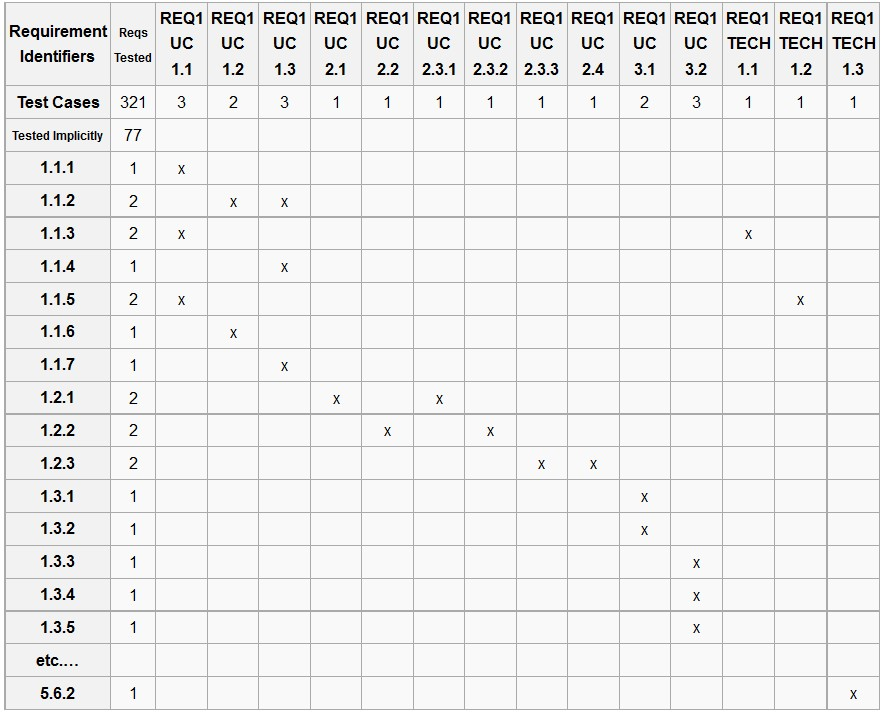
\includegraphics[width=1\linewidth]{TraceabilityMatrix}
\caption{\ttfamily{Traceability Matrix sample}}
\label{fig:TraceabilityMatrix}
\end{figure}

\rindex{\textbf{T}!Traceability}Traceability is the ability to identify related items in documentation and software, such as requirements with associated tests.

A traceability matrix is a document, usually in the form of a table, that correlates any two baselined documents that require a many-to-many relationship to determine the completeness of the relationship.

It is often used with high-level requirements (these often consist of marketing requirements) and detailed requirements of the product to the matching parts of high-level design, detailed design, \rindex{\textbf{T}!Test Plan}test plan, and \rindex{\textbf{T}!Test Case}test cases.

A requirements traceability matrix may be used to check to see if the current project requirements are being met, and to help in the creation of a request for proposal, software requirements specification, various deliverable documents, and project plan tasks.

Common usage is to take the identifier for each of the items of one document and place them in the left column. The identifiers for the other document are placed across the top row. When an item in the left column is related to an item across the top, a mark is placed in the intersecting cell. The number of relationships are added up for each row and each column. This value indicates the mapping of the two items. Zero values indicate that no relationship exists. It must be determined if a relationship must be made. Large values imply that the relationship is too complex and should be simplified.

To ease the creation of traceability matrices, it is advisable to add the relationships to the source documents for both backward traceability and forward traceability. That way, when an item is changed in one baselined document, it's easy to see what needs to be changed in the other.

\section{Usability Testing}
\label{sec:Usability Testing}

Usability testing is a technique used in user-centered interaction design to evaluate a product by testing it on users. This can be seen as an irreplaceable usability practice, since it gives direct input on how real users use the system. This is in contrast with usability inspection methods where experts use different methods to evaluate a user interface without involving users.

Even if it is called 'testing', it doesn't look like usual functional testing, done by QA engineers.

\begin{quote}
 But this is a testing, because it involved some research and it brings information.
\end{quote} 

Usability testing focuses on measuring a human-made product's capacity to meet its intended purpose. Examples of products that commonly benefit from usability testing are foods, consumer products, web sites or web applications, computer interfaces, documents, and devices. Usability testing measures the usability, or ease of use, of a specific object or set of objects, whereas general human-computer interaction studies attempt to formulate universal principles.
\section{Use Case}
\label{sec:Use Case}

In software and systems engineering, a \index{Use Case}\emph{Use Case} is a list of steps, typically defining interactions between a role (known in Unified Modeling Language as an "actor") and a system, to achieve a goal. The actor can be a human, an external system, or time.

In our industry Use Cases become a special form of a \index{Requirements}Requirement.

\begin{quote}
We may say that Requirements evolve in Use Cases.

Or~\textemdash~this is another form of Requirements, nothing to worry about it.

Anyway, Use Cases derive from \index{User Story}User Stories ([p.\pageref{sec:User Story}]).
\end{quote} 

Use Cases have been widely used in modern software engineering over the last two decades. With its iterative and evolutionary nature, use case is also a good fit for agile development.

When you have good Use Cases, you will be able to create a lot of good \index{Test Case}Test Cases.

\section{User Story}
\label{sec:User Story}

A high-level user or business \textbf{requirement} commonly used in agile software development, typically consisting of one or more sentences in the everyday or business language capturing what functionality a user needs, any non-functional criteria, and also includes acceptance criteria.

Like Use Cases ([p.\pageref{sec:Use Case}]), the 'User Story' is a special form of a \rindex{\textbf{R}!Requirements}Requirement ([p.\pageref{sec:Requirement}]).

\section{Verification}
\label{sec:Verification}

This is the basic level of any testing, it comes from the verb \texttt{to verify}.

\index{Verification}Verification is the simplest confirmation of any \emph{expectation} (or assumption) by examination and through provision of objective evidence that specified requirements have been fulfilled.

\textbf{Example}: have a pie. 

\begin{quote}
Or a \emph{borscht}. 

Or a car.
\end{quote}

Verification is the basic checking that this pie can be eaten, and if so, then the quality of the pie is ok.

Sometimes it is more than enough just to be sure, that software does what was expected.

But sometime not.

I am sure, that you will expect, that the pie should be tasty, right?!

\subsection{and Validation}
\label{sec:and Validation}

\index{Validation}Confirmation by examination and through provision of objective evidence that the informal requirements for a specific intended use or application have been fulfilled. 

Any pie can be cooked as expected by recipe, and this can be tested (verified). But even if recipe is only one, the taste of pies will vary from one cook to other. And because it is very hard to set the requirements of 'how to do a tasty pie', this start to lead to informal requirements. And such reqs can be tested only at the \emph{Validation} level.

This two terms are always presented in testing, but they are not declared. 

Any \index{Test Case}test case can be declared as '\textit{This is a validation test}' or '\textit{This test is about verification only}'. But obviously, nobody will ask '\textit{Let's write some validational test cases, please}'.
\section{Version}
\label{sec:Version}

\rindex{\textbf{V}!Version}The versioning is the process of assigning either unique version names or unique version numbers to unique states of computer software. 

Usually the version of a program is presented like this: 

\begin{quote}
ver. \texttt{3.12.242}\end{quote} 

Let's read it:

\begin{description}
 \item[Major release]~\textemdash~\#3. 
 
 The software was developed to the third release.
 
 \item[Minor release]~\textemdash~\#12.
 
 In the third major release was added some functionality. Maybe was added 12 new functions in one day. 
 
 Maybe not, maybe to 11 already existed functions today was the 12. 
 
 Maybe in major release \#3 was added only one new function, with 11 important updates.

 \item[Build]~\textemdash~\#242 \rindex{\textbf{B}!Build}
 
 I can suppose, that someone had a bad day and made 242 bugfixes. Each bugfix increase build numbering with $+1$.
\end{description}

At a fine-grained level, revision control is often used for keeping track of incrementally different versions of electronic information, whether or not this information is computer software.

We can change numbers at any time. Now we have ver. \texttt{3.12.242}. Add one new feature, and this can be ver. \texttt{3.13.0} Apply some small modifications, and we have ver. \texttt{3.13.1} Add one new feature, and here is the ver. \texttt{3.14.0} 

\section{White Box / Black Box Testing}
\label{sec:White Box Black Box Testing}

It is completely not about colors (Black/White), but nobody cares (and clearly will not).

Please, do not share the stupid idea that '\textit{White Box can be done when you look into the source code, and the Black Box can be done when you don't have an acces to source code}'. There are thousand of situations, when you'll look directly into the source code, and you will perform classic Black Box testing.

\begin{quote}
 Later you will realize, that developers understand this 'boxes' better than testers\ldots
\end{quote} 

\index{White Box} \index{Black Box}'White~\&~Black' boxes are just a very convenient \emph{metaphors} (see p.\pageref{sec:Metaphor}) in testing terminology. They perfectly explain the source where tester has searched for ideas to create \index{Test Case}test cases\footnote{Situations to be tested}.

Keep it simple.  As a tester you have to 
\begin{itemize}
\item 
realize what kind of situation may happen when user will start to interact with the application (and which situations can happen, but should not), 
\item 
create these situations one by one and see what's happen.                                                                                                                                                                                                              \end{itemize}

This is the whole \emph{Testing}.

You can have all those situations listed in \index{Requirements}Requirements (p.\pageref{sec:Requirement}). If it so, then you are a lucky bastard (or you are in army). But for a mass-market application (any modern website) you will be out of this luxury. So, you have to invent or discover them by yourself. How to do it?

Sometimes you can know exactly how your app should working. You will imagine situations (so \index{Test Case}test cases will appear), and you will swtich to the illuminated zone — the 'White box' metaphor.

\begin{quote}
Doesn't matter, where you will bring this information. You can read requirements? Now you know. You can read source code? Now you know. You can ask someone who knows about it? Now you know too. 
\end{quote} 

Sometimes you know nothing, and you slide to a darker zone (the 'Black box' metaphor), where you have to often suppose what should happen than knowing exactly. You should explore, like 'Let's provide to this input field several characters and see how the software will react to it\ldots'.

As you can see, the \emph{researching} (or, sometimes, exploration) is not a testing. They are always close, but they are not the same.

\begin{quote}
In testing you ALWAYS know the \index{Expected result}expected result. And you can compare it with \index{Actual result}actual result.

In researching you may be blind about the expected result, but when you will know —  you can test. That's why texting and researching are always close.
\end{quote} 

\subsection{Why 'boxes'}

The software, in the eyes of a tester, is like a box with some magic inside.

You don't know exactly how and why the coffe-machine works, but you can interact with it. The 'box' is 'black'.

You may not understand how and why an engine works (or how it looks like), but you can drive a car. The 'box' is 'black'.

You don't know what to do with your miserable life, but you still live it. The 'box' is 'black'.

And if you know How and Why it works — the box became 'transparent' for you.

\begin{quote}
That's why someone can say 'A glass box', or even 'The transparent box', opposite to 'The black box'.                                                                                                                                                                                       \end{quote} 

\subsection{What about strategies}

\index{Glenford J. Myers}Bearded old school testers (covered by bearded old school developers) claims that the 'White/Black Box Testing' is a \emph{strategy}\footnote{<<Art of Software Testing>> by Glenford J. Myers, 1979, John Wiley \& Sons, Inc.} (see  p.\pageref{sec:Strategy}). And if this is a strategy, then we can combine the 'black' and 'white' to the 'gray box'.

Well, it really looks alike. But no.

And there are no 'gray' boxes in testing.

\printindex

% Финиш
\newpage
\thispagestyle{empty} 
	\vspace*{\fill}
	\begingroup
	\centering
		{\fontsize{150}{160}\selectfont THE END}
	\endgroup
	\vspace*{\fill}

\end{document}
